\documentclass[journal]{IEEEtran}
%
% If IEEEtran.cls has not been installed into the LaTeX system files,
% manually specify the path to it like:
% \documentclass[journal]{../sty/IEEEtran}





% Some very useful LaTeX packages include:
% (uncomment the ones you want to load)


% *** MISC UTILITY PACKAGES ***
%
%\usepackage{ifpdf}
% Heiko Oberdiek's ifpdf.sty is very useful if you need conditional
% compilation based on whether the output is pdf or dvi.
% usage:
% \ifpdf
%   % pdf code
% \else
%   % dvi code
% \fi
% The latest version of ifpdf.sty can be obtained from:
% http://www.ctan.org/pkg/ifpdf
% Also, note that IEEEtran.cls V1.7 and later provides a builtin
% \ifCLASSINFOpdf conditional that works the same way.
% When switching from latex to pdflatex and vice-versa, the compiler may
% have to be run twice to clear warning/error messages.


\usepackage{graphicx}
\usepackage{url}
\usepackage{mathtools}
\usepackage{CJK}
\usepackage{subfigure} 
\usepackage{cite}
\usepackage{graphicx}

\usepackage{floatrow}
\floatsetup[table]{capposition=top}
\newfloatcommand{capbtabbox}{table}[][\FBwidth]

% *** CITATION PACKAGES ***
%
%\usepackage{cite}
% cite.sty was written by Donald Arseneau
% V1.6 and later of IEEEtran pre-defines the format of the cite.sty package
% \cite{} output to follow that of the IEEE. Loading the cite package will
% result in citation numbers being automatically sorted and properly
% "compressed/ranged". e.g., [1], [9], [2], [7], [5], [6] without using
% cite.sty will become [1], [2], [5]--[7], [9] using cite.sty. cite.sty's
% \cite will automatically add leading space, if needed. Use cite.sty's
% noadjust option (cite.sty V3.8 and later) if you want to turn this off
% such as if a citation ever needs to be enclosed in parenthesis.
% cite.sty is already installed on most LaTeX systems. Be sure and use
% version 5.0 (2009-03-20) and later if using hyperref.sty.
% The latest version can be obtained at:
% http://www.ctan.org/pkg/cite
% The documentation is contained in the cite.sty file itself.






% *** GRAPHICS RELATED PACKAGES ***
%
\ifCLASSINFOpdf
  % \usepackage[pdftex]{graphicx}
  % declare the path(s) where your graphic files are
  % \graphicspath{{../pdf/}{../jpeg/}}
  % and their extensions so you won't have to specify these with
  % every instance of \includegraphics
  % \DeclareGraphicsExtensions{.pdf,.jpeg,.png}
\else
  % or other class option (dvipsone, dvipdf, if not using dvips). graphicx
  % will default to the driver specified in the system graphics.cfg if no
  % driver is specified.
  % \usepackage[dvips]{graphicx}
  % declare the path(s) where your graphic files are
  % \graphicspath{{../eps/}}
  % and their extensions so you won't have to specify these with
  % every instance of \includegraphics
  % \DeclareGraphicsExtensions{.eps}
\fi
% graphicx was written by David Carlisle and Sebastian Rahtz. It is
% required if you want graphics, photos, etc. graphicx.sty is already
% installed on most LaTeX systems. The latest version and documentation
% can be obtained at: 
% http://www.ctan.org/pkg/graphicx
% Another good source of documentation is "Using Imported Graphics in
% LaTeX2e" by Keith Reckdahl which can be found at:
% http://www.ctan.org/pkg/epslatex
%
% latex, and pdflatex in dvi mode, support graphics in encapsulated
% postscript (.eps) format. pdflatex in pdf mode supports graphics
% in .pdf, .jpeg, .png and .mps (metapost) formats. Users should ensure
% that all non-photo figures use a vector format (.eps, .pdf, .mps) and
% not a bitmapped formats (.jpeg, .png). The IEEE frowns on bitmapped formats
% which can result in "jaggedy"/blurry rendering of lines and letters as
% well as large increases in file sizes.
%
% You can find documentation about the pdfTeX application at:
% http://www.tug.org/applications/pdftex





% *** MATH PACKAGES ***
%
%\usepackage{amsmath}
% A popular package from the American Mathematical Society that provides
% many useful and powerful commands for dealing with mathematics.
%
% Note that the amsmath package sets \interdisplaylinepenalty to 10000
% thus preventing page breaks from occurring within multiline equations. Use:
%\interdisplaylinepenalty=2500
% after loading amsmath to restore such page breaks as IEEEtran.cls normally
% does. amsmath.sty is already installed on most LaTeX systems. The latest
% version and documentation can be obtained at:
% http://www.ctan.org/pkg/amsmath





% *** SPECIALIZED LIST PACKAGES ***
%
%\usepackage{algorithmic}
% algorithmic.sty was written by Peter Williams and Rogerio Brito.
% This package provides an algorithmic environment fo describing algorithms.
% You can use the algorithmic environment in-text or within a figure
% environment to provide for a floating algorithm. Do NOT use the algorithm
% floating environment provided by algorithm.sty (by the same authors) or
% algorithm2e.sty (by Christophe Fiorio) as the IEEE does not use dedicated
% algorithm float types and packages that provide these will not provide
% correct IEEE style captions. The latest version and documentation of
% algorithmic.sty can be obtained at:
% http://www.ctan.org/pkg/algorithms
% Also of interest may be the (relatively newer and more customizable)
% algorithmicx.sty package by Szasz Janos:
% http://www.ctan.org/pkg/algorithmicx




% *** ALIGNMENT PACKAGES ***
%
%\usepackage{array}
% Frank Mittelbach's and David Carlisle's array.sty patches and improves
% the standard LaTeX2e array and tabular environments to provide better
% appearance and additional user controls. As the default LaTeX2e table
% generation code is lacking to the point of almost being broken with
% respect to the quality of the end results, all users are strongly
% advised to use an enhanced (at the very least that provided by array.sty)
% set of table tools. array.sty is already installed on most systems. The
% latest version and documentation can be obtained at:
% http://www.ctan.org/pkg/array


% IEEEtran contains the IEEEeqnarray family of commands that can be used to
% generate multiline equations as well as matrices, tables, etc., of high
% quality.




% *** SUBFIGURE PACKAGES ***
%\ifCLASSOPTIONcompsoc
%  \usepackage[caption=false,font=normalsize,labelfont=sf,textfont=sf]{subfig}
%\else
%  \usepackage[caption=false,font=footnotesize]{subfig}
%\fi
% subfig.sty, written by Steven Douglas Cochran, is the modern replacement
% for subfigure.sty, the latter of which is no longer maintained and is
% incompatible with some LaTeX packages including fixltx2e. However,
% subfig.sty requires and automatically loads Axel Sommerfeldt's caption.sty
% which will override IEEEtran.cls' handling of captions and this will result
% in non-IEEE style figure/table captions. To prevent this problem, be sure
% and invoke subfig.sty's "caption=false" package option (available since
% subfig.sty version 1.3, 2005/06/28) as this is will preserve IEEEtran.cls
% handling of captions.
% Note that the Computer Society format requires a larger sans serif font
% than the serif footnote size font used in traditional IEEE formatting
% and thus the need to invoke different subfig.sty package options depending
% on whether compsoc mode has been enabled.
%
% The latest version and documentation of subfig.sty can be obtained at:
% http://www.ctan.org/pkg/subfig




% *** FLOAT PACKAGES ***
%
%\usepackage{fixltx2e}
% fixltx2e, the successor to the earlier fix2col.sty, was written by
% Frank Mittelbach and David Carlisle. This package corrects a few problems
% in the LaTeX2e kernel, the most notable of which is that in current
% LaTeX2e releases, the ordering of single and double column floats is not
% guaranteed to be preserved. Thus, an unpatched LaTeX2e can allow a
% single column figure to be placed prior to an earlier double column
% figure.
% Be aware that LaTeX2e kernels dated 2015 and later have fixltx2e.sty's
% corrections already built into the system in which case a warning will
% be issued if an attempt is made to load fixltx2e.sty as it is no longer
% needed.
% The latest version and documentation can be found at:
% http://www.ctan.org/pkg/fixltx2e


%\usepackage{stfloats}
% stfloats.sty was written by Sigitas Tolusis. This package gives LaTeX2e
% the ability to do double column floats at the bottom of the page as well
% as the top. (e.g., "\begin{figure*}[!b]" is not normally possible in
% LaTeX2e). It also provides a command:
%\fnbelowfloat
% to enable the placement of footnotes below bottom floats (the standard
% LaTeX2e kernel puts them above bottom floats). This is an invasive package
% which rewrites many portions of the LaTeX2e float routines. It may not work
% with other packages that modify the LaTeX2e float routines. The latest
% version and documentation can be obtained at:
% http://www.ctan.org/pkg/stfloats
% Do not use the stfloats baselinefloat ability as the IEEE does not allow
% \baselineskip to stretch. Authors submitting work to the IEEE should note
% that the IEEE rarely uses double column equations and that authors should try
% to avoid such use. Do not be tempted to use the cuted.sty or midfloat.sty
% packages (also by Sigitas Tolusis) as the IEEE does not format its papers in
% such ways.
% Do not attempt to use stfloats with fixltx2e as they are incompatible.
% Instead, use Morten Hogholm'a dblfloatfix which combines the features
% of both fixltx2e and stfloats:
%
% \usepackage{dblfloatfix}
% The latest version can be found at:
% http://www.ctan.org/pkg/dblfloatfix




%\ifCLASSOPTIONcaptionsoff
%  \usepackage[nomarkers]{endfloat}
% \let\MYoriglatexcaption\caption
% \renewcommand{\caption}[2][\relax]{\MYoriglatexcaption[#2]{#2}}
%\fi
% endfloat.sty was written by James Darrell McCauley, Jeff Goldberg and 
% Axel Sommerfeldt. This package may be useful when used in conjunction with 
% IEEEtran.cls'  captionsoff option. Some IEEE journals/societies require that
% submissions have lists of figures/tables at the end of the paper and that
% figures/tables without any captions are placed on a page by themselves at
% the end of the document. If needed, the draftcls IEEEtran class option or
% \CLASSINPUTbaselinestretch interface can be used to increase the line
% spacing as well. Be sure and use the nomarkers option of endfloat to
% prevent endfloat from "marking" where the figures would have been placed
% in the text. The two hack lines of code above are a slight modification of
% that suggested by in the endfloat docs (section 8.4.1) to ensure that
% the full captions always appear in the list of figures/tables - even if
% the user used the short optional argument of \caption[]{}.
% IEEE papers do not typically make use of \caption[]'s optional argument,
% so this should not be an issue. A similar trick can be used to disable
% captions of packages such as subfig.sty that lack options to turn off
% the subcaptions:
% For subfig.sty:
% \let\MYorigsubfloat\subfloat
% \renewcommand{\subfloat}[2][\relax]{\MYorigsubfloat[]{#2}}
% However, the above trick will not work if both optional arguments of
% the \subfloat command are used. Furthermore, there needs to be a
% description of each subfigure *somewhere* and endfloat does not add
% subfigure captions to its list of figures. Thus, the best approach is to
% avoid the use of subfigure captions (many IEEE journals avoid them anyway)
% and instead reference/explain all the subfigures within the main caption.
% The latest version of endfloat.sty and its documentation can obtained at:
% http://www.ctan.org/pkg/endfloat
%
% The IEEEtran \ifCLASSOPTIONcaptionsoff conditional can also be used
% later in the document, say, to conditionally put the References on a 
% page by themselves.




% *** PDF, URL AND HYPERLINK PACKAGES ***
%
%\usepackage{url}
% url.sty was written by Donald Arseneau. It provides better support for
% handling and breaking URLs. url.sty is already installed on most LaTeX
% systems. The latest version and documentation can be obtained at:
% http://www.ctan.org/pkg/url
% Basically, \url{my_url_here}.




% *** Do not adjust lengths that control margins, column widths, etc. ***
% *** Do not use packages that alter fonts (such as pslatex).         ***
% There should be no need to do such things with IEEEtran.cls V1.6 and later.
% (Unless specifically asked to do so by the journal or conference you plan
% to submit to, of course. )


% correct bad hyphenation here
\hyphenation{op-tical net-works semi-conduc-tor}



\begin{document}
%
% paper title
% Titles are generally capitalized except for words such as a, an, and, as,
% at, but, by, for, in, nor, of, on, or, the, to and up, which are usually
% not capitalized unless they are the first or last word of the title.
% Linebreaks \\ can be used within to get better formatting as desired.
% Do not put math or special symbols in the title.
\title{MPDNet: Multimodal Pneumonia Detection Network Simulating Clinical Diagnosis Process}
%
%
% author names and IEEE memberships
% note positions of commas and nonbreaking spaces ( ~ ) LaTeX will not break
% a structure at a ~ so this keeps an author's name from being broken across
% two lines.
% use \thanks{} to gain access to the first footnote area
% a separate \thanks must be used for each paragraph as LaTeX2e's \thanks
% was not built to handle multiple paragraphs
%

\author{Qiuli~Wang,
        Zhihuan~Li,
        Dan~Yang\IEEEauthorrefmark{1},
        Chen~Liu\IEEEauthorrefmark{1},
        Xiaohong~Zhang\IEEEauthorrefmark{1}% <-this % stops a space

\thanks{This work was partially supported by the National Natural Science Foundation of China (Grant No. 61772093), the Chongqing Major Theme Projects (Grant Nos. cstc2018jszx-cyztzxX0017, cstc2017zdcy-zdzx0077), and Fundamental Research Funds for the Central Universities (Grant Nos. CDJZR14105501, CDXYRJ0011). Asterisks indicate corresponding authors.
}
\thanks{Q.~Wang Z.~Li and D.~Yang are with the School of Big Data \& Software Engineering, Chongqing University, Chongqing 401331, China. E-mail: dyang@cqu.edu.cn.}
\thanks{L.~Chen is with the Radiology Department, The First Affiliated Hospital of Army Medical University, 400032, Chongqing, China. E-mail:cqliuchen@foxmail.com. }
\thanks{X. Zhang is with the Key Laboratory of Dependable Service Computing in Cyber Physical Society, Ministry of Education, Chongqing University, Chongqing 400044, China, also with the School of Software Engineering, Chongqing University, Chongqing 401331, China, and also with the State Key laboratory of Coal Mine Disaster Dynamics and Control, Chongqing University, Chongqing 400044, China. E-mail: xhongz@cqu.edu.cn.}

% <-this % stops a space
}

% note the % following the last \IEEEmembership and also \thanks - 
% these prevent an unwanted space from occurring between the last author name
% and the end of the author line. i.e., if you had this:
% 
% \author{....lastname \thanks{...} \thanks{...} }
%                     ^------------^------------^----Do not want these spaces!
%
% a space would be appended to the last name and could cause every name on that
% line to be shifted left slightly. This is one of those "LaTeX things". For
% instance, "\textbf{A} \textbf{B}" will typeset as "A B" not "AB". To get
% "AB" then you have to do: "\textbf{A}\textbf{B}"
% \thanks is no different in this regard, so shield the last } of each \thanks
% that ends a line with a % and do not let a space in before the next \thanks.
% Spaces after \IEEEmembership other than the last one are OK (and needed) as
% you are supposed to have spaces between the names. For what it is worth,
% this is a minor point as most people would not even notice if the said evil
% space somehow managed to creep in.



% The paper headers
\markboth{ }%
{Q.~Wang \MakeLowercase{\textit{et al.}}: MPDNet}
% The only time the second header will appear is for the odd numbered pages
% after the title page when using the twoside option.
% 
% *** Note that you probably will NOT want to include the author's ***
% *** name in the headers of peer review papers.                   ***
% You can use \ifCLASSOPTIONpeerreview for conditional compilation here if
% you desire.


% If you want to put a publisher's ID mark on the page you can do it like
% this:
%\IEEEpubid{0000--0000/00\$00.00~\copyright~2015 IEEE}
% Remember, if you use this you must call \IEEEpubidadjcol in the second
% column for its text to clear the IEEEpubid mark.



% use for special paper notices
%\IEEEspecialpapernotice{(Invited Paper)}




% make the title area
\maketitle

% As a general rule, do not put math, special symbols or citations
% in the abstract or keywords.
\begin{abstract}
    \emph{Objective:} Pneumonia detection is one of the most crucial steps in the pneumonia diagnosing system. Clinical information of patients plays an essential role in the detection of pneumonia, but few models consider this information. In this paper, a Multimodal Pneumonia Detection Network (MPDNet) is described for clinical pneumonia detection.
    \emph{Method:} MPDNet simulates clinical pneumonia detection process and considers multimodal data: three-channel CT images,  chief complaints, patient age, and gender. 
    (a) MPDNet firstly extracts visual features from three-channel (Lung Window, High Attenuation, Low Attenuation) images, which are transformed from one-channel grey level CT images. Different channels can provide supplementary features to each other and give qualitative information for pneumonia detection. A dedicated Recurrent CNN (RCNN) is used to extract 3D visual features from three-channel images and reduce the need for calculation resources.
    (b) Then MPDNet extracts information about lesion location, symptoms, or how long patients have been ill from chief complaints, which enhances visual features extracted from CT images. A Long Short Term Memory(LSTM) network is used to analyze the semantic features of patient chief complaints. 
    (c) Moreover, MPDNet uses priori information provided by age and gender to improve the decision-making process.
    In MPDNet, we incorporate CT visual features, complaint semantic features, patient age, and gender to calculate joint distribution and simulates clinical pneumonia detection.
    \emph{Results:} The proposed MPDNet has been extensively validated in 1002 clinical cases from The First Affiliated Hospital of Army Medical University. Our network achieves 0.945 in accuracy and has a very balanced performance in sensitivity and specificity. As far as we know, we are the first to detect pneumonic cases using large scale clinical multimodal data.
    \emph{Conclusion:} Our method demonstrates that multimodal data provides more abundant information than image data only and gets very convincing results.
    \emph{Significance:} While MPDNet is tailored for pneumonia detection, it can be extended and include more multimodal clinical data to give out more reliable and explainable detection results.
\end{abstract}

% Note that keywords are not normally used for peerreview papers.
\begin{IEEEkeywords}
    Multimodal Data, Pneumonia Detection, Computed Tomography (CT), Computer-Aided Detection and Diagnosis (CAD)
\end{IEEEkeywords}



% For peer review papers, you can put extra information on the cover
% page as needed:
% \ifCLASSOPTIONpeerreview
% \begin{center} \bfseries EDICS Category: 3-BBND \end{center}
% \fi
%
% For peerreview papers, this IEEEtran command inserts a page break and
% creates the second title. It will be ignored for other modes.
\IEEEpeerreviewmaketitle

\newpage
\section{Introduction}
\label{intro}
% The very first letter is a 2 line initial drop letter followed
% by the rest of the first word in caps.
% 
% form to use if the first word consists of a single letter:
% \IEEEPARstart{A}{demo} file is ....
% 
% form to use if you need the single drop letter followed by
% normal text (unknown if ever used by the IEEE):
% \IEEEPARstart{A}{}demo file is ....
% 
% Some journals put the first two words in caps:
% \IEEEPARstart{T}{his demo} file is ....
% 
% Here we have the typical use of a "T" for an initial drop letter
% and "HIS" in caps to complete the first word.

\IEEEPARstart{P}{neumonia} is a prevalent thoracic disease in daily life. In clinical practice, multimodal data plays a key role in the decision-making process. Radiologists need to consider multimodal information to decide on the next treatment plan. As a result, radiologists from major hospitals have a heavy burden of work. Thus, developing a fast, robust, and accurate CAD system to perform automated detection of pneumonia is meaningful and vital. 
\begin{figure*}[htbp]
    \centering
    \subfigure[Clinical Practice of Pneumonia Diagnosis]{
    \begin{minipage}[t]{1\linewidth}
    \centering
    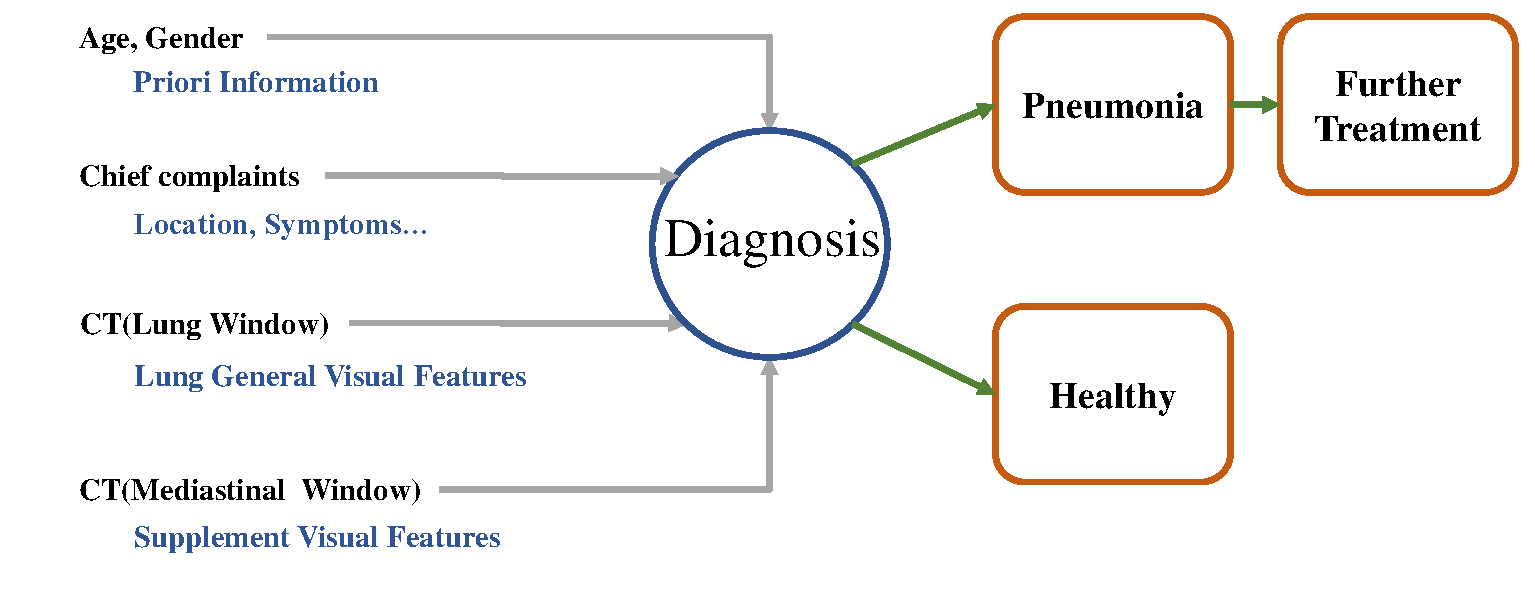
\includegraphics[width=5.5in]{MPD1.pdf}
    %\caption{fig1}
    \end{minipage}%
    }

    \subfigure[Architecture of MPDNet]{
    \begin{minipage}[t]{1\linewidth}
    \centering
    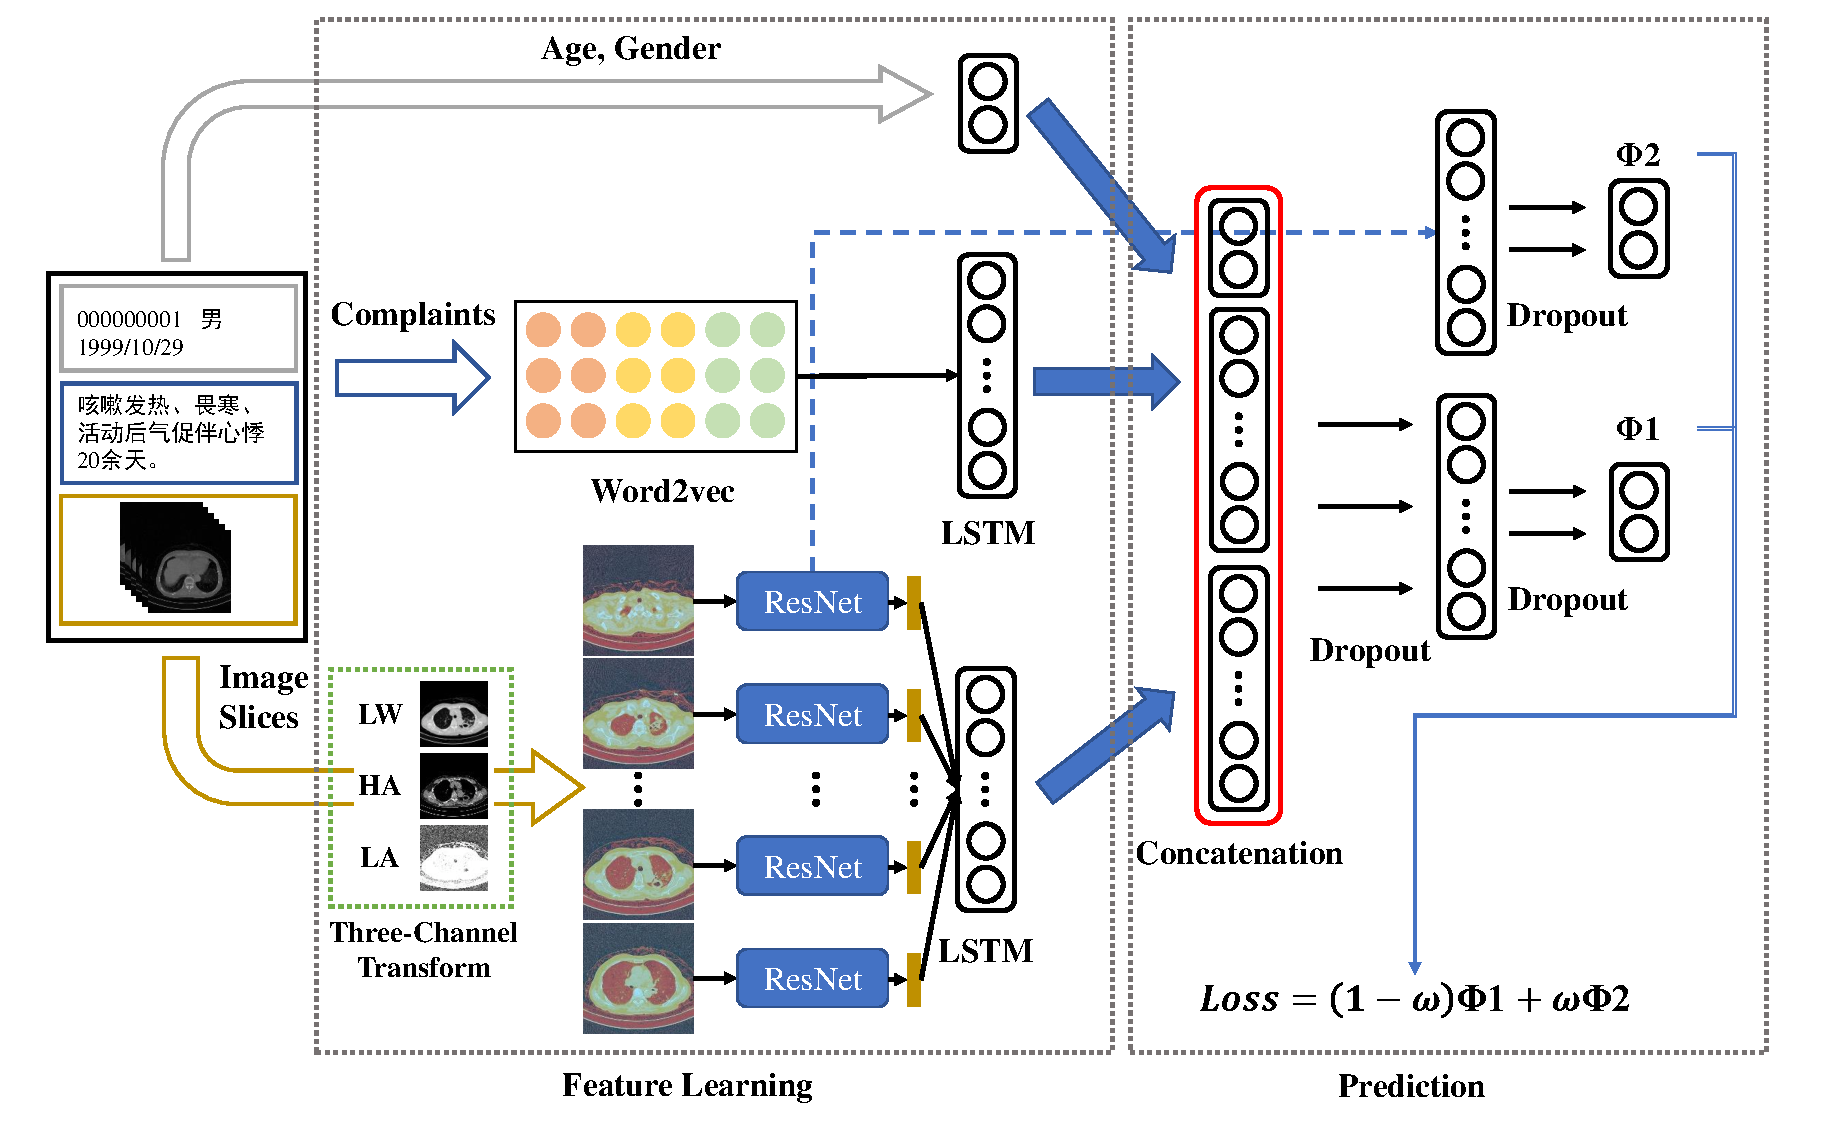
\includegraphics[width=6in]{MPD2.pdf}
    %\caption{fig2}
    \end{minipage}%
    }
    \centering
    \caption{(a) shows the clinical practice of detecting pneumonia. Age and gender provide priori information; chief complaints provide information like symptoms, location of pain; different CT windows provide visual features. (b) shows the architecture of MPDNet. The black box in the left indicates raw information from the hospital. In the black box, the information in the grey rectangle is about age and gender; the information in the blue rectangle is chief complaints; the information in yellow rectangle is CT image data. Chief complaints will be transformed into matrices by Word2vec and analyze by one LSTM network. Images will be fed into RCNN. LW (Lung Window), HA (High Attenuation), LA (Low Attenuation) in the green box represent three image window: lung window, high attenuation window, and low attenuation window. Age and gender will be treated as two additional features. These three kinds of information will be concatenated in the red rectangle and simulate the clinical process.
    }
    \label{MMDD}
    \end{figure*}

Many research works have devoted efforts in pneumonia detection, monitoring and diagnosing like \cite{Shin2016Learning, deepika2018classification, iakovidis2012image}.
Hoo-Chang Shin \cite{Shin2016Learning} proposed a method which used CNN to extract features from chest X-Ray and used LSTM \cite{hochreiter1997long} to generated MeSH \cite{timmurphy.org} terms for chest X-Ray. In 2017, Xiaosong Wang et al. \cite{Wang2017ChestX} provided hospital-scale chest X-ray database ChestX-ray8, which contained eight common thoracic diseases. This database allowed researchers to use deeper neural networks to analyze thoracic diseases. They tested different pre-trained CNN models on this dataset. Experiments showed that ResNet50 achieved the highest AUROC score of 0.6333 in classifying pneumonia. They also provided ChestX-ray14, which contains more kinds of thoracic diseases.
Based on this database, later in 2017, Yao et al. \cite{yao2017learning} achieved AUROC of 0.713 in classifying pneumonia using DenseNet Image Encoder. Pranav Rajpurkar, Andrew Y. Ng et al. \cite{Rajpurkar2017CheXNet} developed CheXnet with 121 convolutional layers and achieved AUROC 0.7680 in pneumonia classification.
In 2018, Xiaosong Wang et al. \cite{Wang2018TieNet} proposed TieNet, which could classify the chest X-Rays into different diseases and generate the report at the same time. In TieNet, CNN was used to capture features of chest X-Rays, RNN learned these features and generated reports based on attention mechanism, which could help the model to focus on different parts of chest X-rays alone with the generation of reports. In the pneumonia classification problem, they achieved 0.947 in AUROC based on reports, but they only reached 0.917 in AUROC on hand-labeled data. 

Studies above have something in common. First of all, they are designed for chest X-Rays. Chest X-rays used to be the best available method for detect pneumonia, played a crucial role in clinical care and epidemiological studies \cite{Franquet2001Imaging, Thomas2005Standardized}. 
However, compared to chest X-rays, CT scans have a more unobstructed view of patients' bodies and allow visualization of 3D lung structures \cite{korfiatis2009texture}, since bones, skin, vessels, mediastinal and lung tissues may cause overlapping shadows in chest X-ray and cause misdiagnosis. CT can help to diagnose pneumonia in early-stage and avoid delayed treatments.
Extensive studies show that 3D CNN is the best choice for keeping 3D spatial information in CT \cite{Yorozu1987Electron}. However, 3D CNN cannot be applied to raw CT data directly since it will bring a heavy burden to computers. Radiologists need to measure the lesions accurately, so we cannot reduce the size of images by resizing at will.
Second, these models are not designed following the radiologists' diagnosing process but for the convenience of computer vision studies and deep learning model training. For models like CheXnet, image information is the key to models. Few of them combine image visual features with clinical information. 
Models like TieNet do combine image visual features with descriptions about images written by radiologists. We believe using descriptions about images written by radiologists to improve models is not entirely convincing since descriptions like `Findings' and `Impressions' sometimes include diagnosis conclusions.
However, there have been many studies try to analyze multimodal data like \cite{hu2019deep, xiao2018alternating}. Multimodal data can be multimodal images \cite{dou2016multilevel} or multimodal data source. 
Patients' chief complaints are valuable information when doctors are making decisions \cite{wu2018master}, since chief complaints are patients' direct feeling about their physical condition, telling us the patients' pain location, symptoms and how long have they been ill. Moreover, information about age and gender can provide priori information\cite{xiaojian2011analysis, huang2014design}. However, as far as we know, few studies use this information to improve CAD systems for pneumonia. 

In general, there are two major drawbacks of existing CAD systems for pneumonia: (1) They cannot handle raw CT scans, which allows visualization of lung structures; (2) Few studies consider multimodal clinical information like patients' chief complaints, which is a conflict to clinical practice.

To address such drawbacks, we propose a novel Multimodal Pneumonia Detection Network (MPDNet) and simulate clinical pneumonia detection. The architecture of MPDNet is shown in Fig~\ref{MMDD}. We use raw data collected from The First Affiliated Hospital of Army Medical University. Each case contains not only CT image information but also clinical information about patient gender, age, and chief complaints. 

Herein, (i) each CT image will be transformed into a three-channel image with three windows: Lung Window(LW), High Attenuation(HA) and Low Attenuation(LA). LW provides visual features of normal lung tissues, HA provides visual features of abnormal increase in lung density, LA provides visual features of abnormal decrease in lung density. Three channels complement each other, which not only maintains the ability to extract information from normal lung tissues but also increases the ability to extract information from abnormal lung tissues.
(ii) We also include clinical data in our MPDNet. Chief complaints can provide the location of pain, symptoms, and how long have patients been ill. This information is related to the CT image and enhances the visual features extracted from CT. 
(iii) Information about age and gender can provide priori information since patients of different age and gender have differences in the morphology of the thoracic cavity and lungs. 
(iv) To reduce the burden of calculation, we treat CT slices as short video frames and a Recurrent Convolutional Neural Network (RCNN) is used to capture visual features from CT slices. RCNN uses a 2D CNN to capture visual features from each 2D slice, and LSTM captures relationships between slices. We use another LSTM to analyze semantics from chief complaints. Information about age and gender will be treated as two extra variables. Our model MPDNet, as shown in Fig~\ref{MMDD}, will learn a joint distribution of all features above and gives out the final detecting results.

The remainder of the manuscript is organized as follows. 
Section~\ref{datasetprocessing} describes the prepare of dataset and pre-process steps.
Section~\ref{MPDNetwork} describes the architecture of MPDNet and details of our model.
Section~\ref{experiments} reports our experimental results. We further discusses some key points of proposed model and some phenomenons shown during experiments in this section.
Our conclusions are summarized in section~\ref{conclude}.


\section{Dataset Processing}
\label{datasetprocessing}
\subsection{CT Image Data and Multimodal Data Generation}
\label{ctimagedata}
Because of the shortage of public available CT dataset for pneumonia, we use the raw data from the Radiology Department of The First Affiliated Hospital of Army Medical University. We get 1036 cases of CT (842 pneumonic cases, 464 healthy cases) from hospital PACS (Picture Archiving and Communication Systems). Raw data from the hospital may have more than one series of images, and each series has specific data types, image windows, or view angles. 
Generally speaking, radiologists and doctors will use the series under lung window with the smallest `Slice Thickness', but for deep learning models, each case can only have one series. So we design a protocol to pick up specific series for us.

First of all, we eliminate these cases which start scanning from the middle of the chest. Then we pick up the best series from the whole cases according to the following requirements:

(a) We choose the series with the specific `Convolution Kernel'. Different `Convolution Kernel' may have different data types or different image windows, as shown in Fig~\ref{Bs}. We need to notice that these names of `Convolution Kernel' vary between hospitals and CT equipment, so if you want to adopt this protocol, you need to observe `Convolution Kernel' in your environment. In our study, we choose `B31f', `I31f 3', `B70f', `B80f', `B70s'. We notice that in the Radiology Department of The First Affiliated Hospital of Army Medical University, `B70s' is the most common parameter used in clinical which contains 620 cases.

\begin{figure}[t]
    \centerline{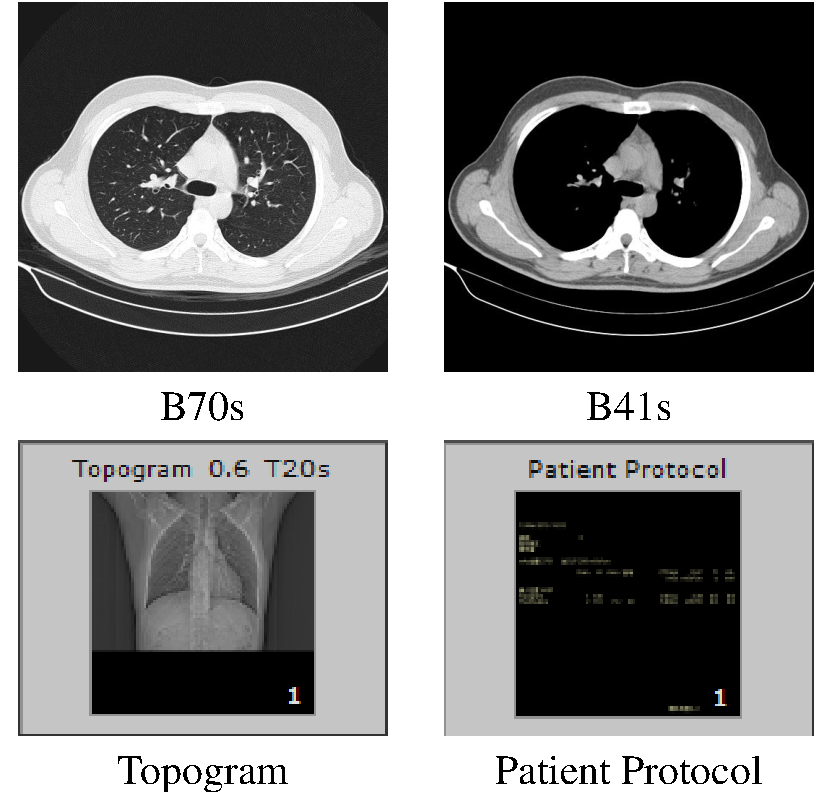
\includegraphics[width=80mm]{Bs.pdf}}
    \vspace{-0cm}
    \caption{Scans under Different `Convolutional Kernel'. Slice under `B70s' has clearer view of lungs, slice under `B41s' has a more unobstructed view of the heart. `Patient Protocol' and `Topogram' contain some basic parameters of CT equipment or information about radiologists, which are not suitable for CNN.}
    \vspace{-0cm}
    \label{Bs}
    \end{figure}

(b) We remove series like `Patient Protocol', `Topogram'. These series, as shown in Fig~\ref{Bs}, contain some basic parameters and information about CT equipment.

(c) We calculate `Slice Thickness' of each series, and keep the series with the smallest `Slice Thickness', since small thickness may keep more detailed information about body structure. 

(d) If there were more than one series meet the last two requirements, we would keep the series with the largest number of slices, which could have a larger span of view.
\begin{figure*}[htbp]
    \centering
    \subfigure[Data Pre-precess for CT Scans]{
    \begin{minipage}[t]{1\linewidth}
    \centering
    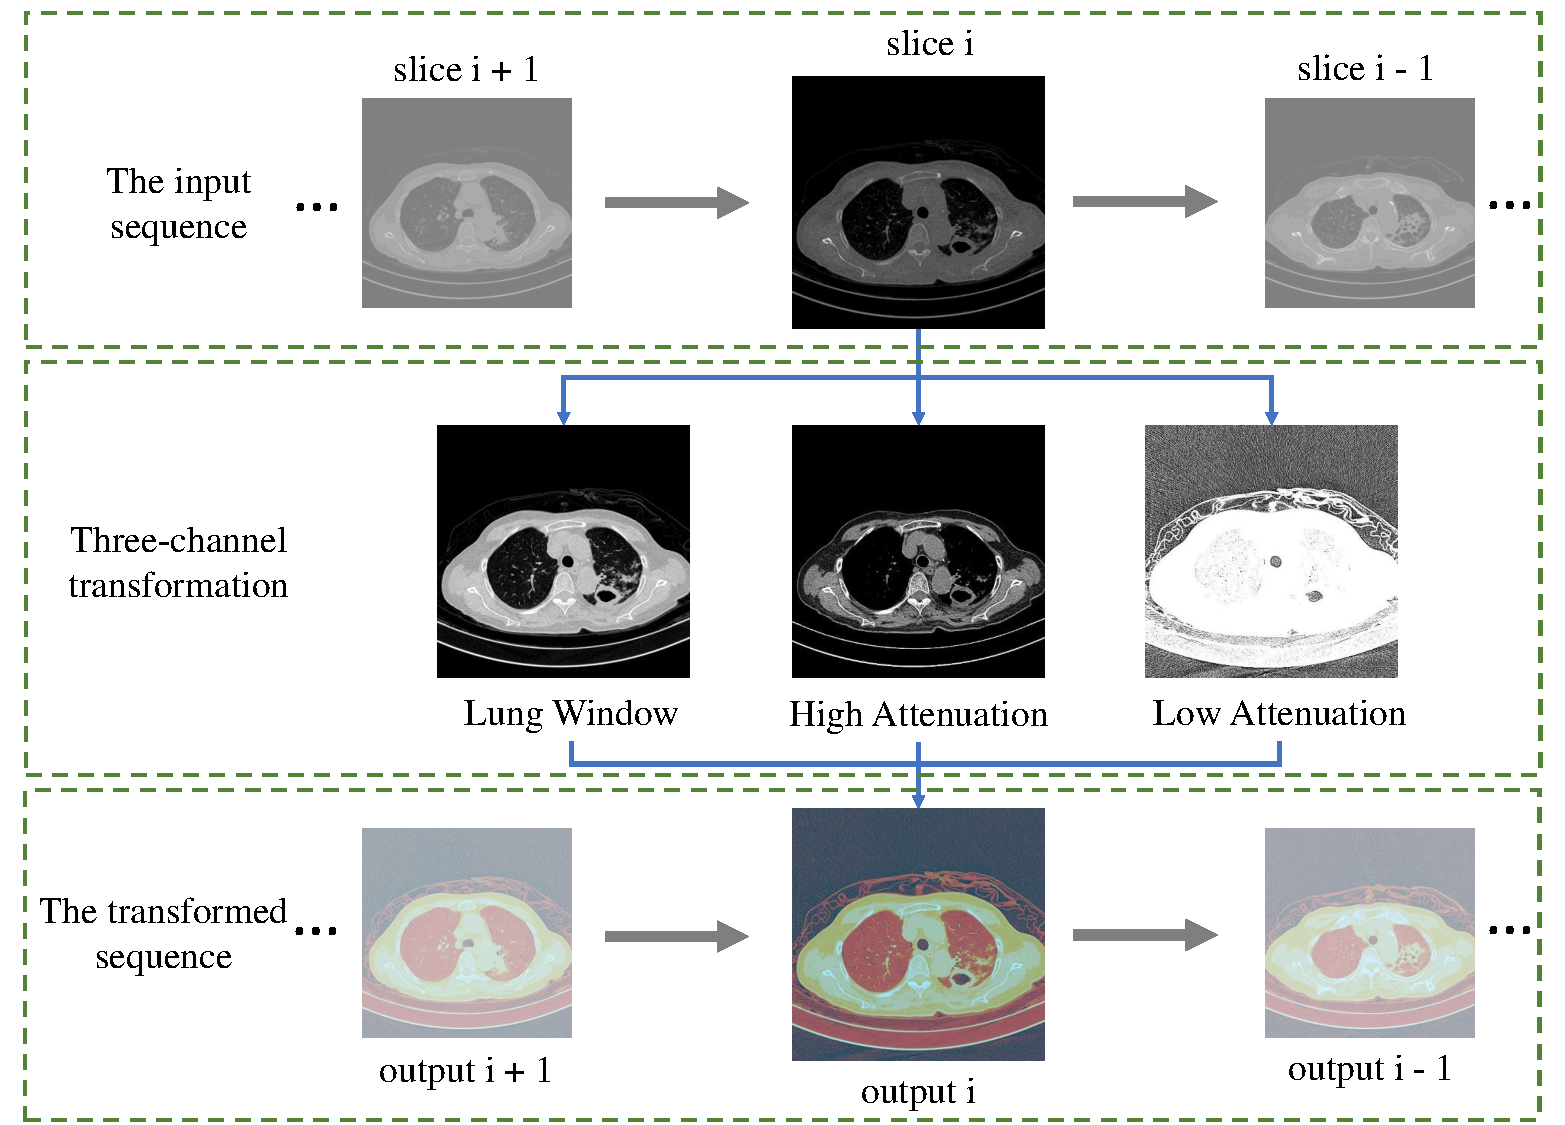
\includegraphics[width=5.5in]{3channel1.pdf}
    %\caption{fig1}
    \end{minipage}%
    }%

    \subfigure[Three-Channel Images]{
    \begin{minipage}[t]{1\linewidth}
    \centering
    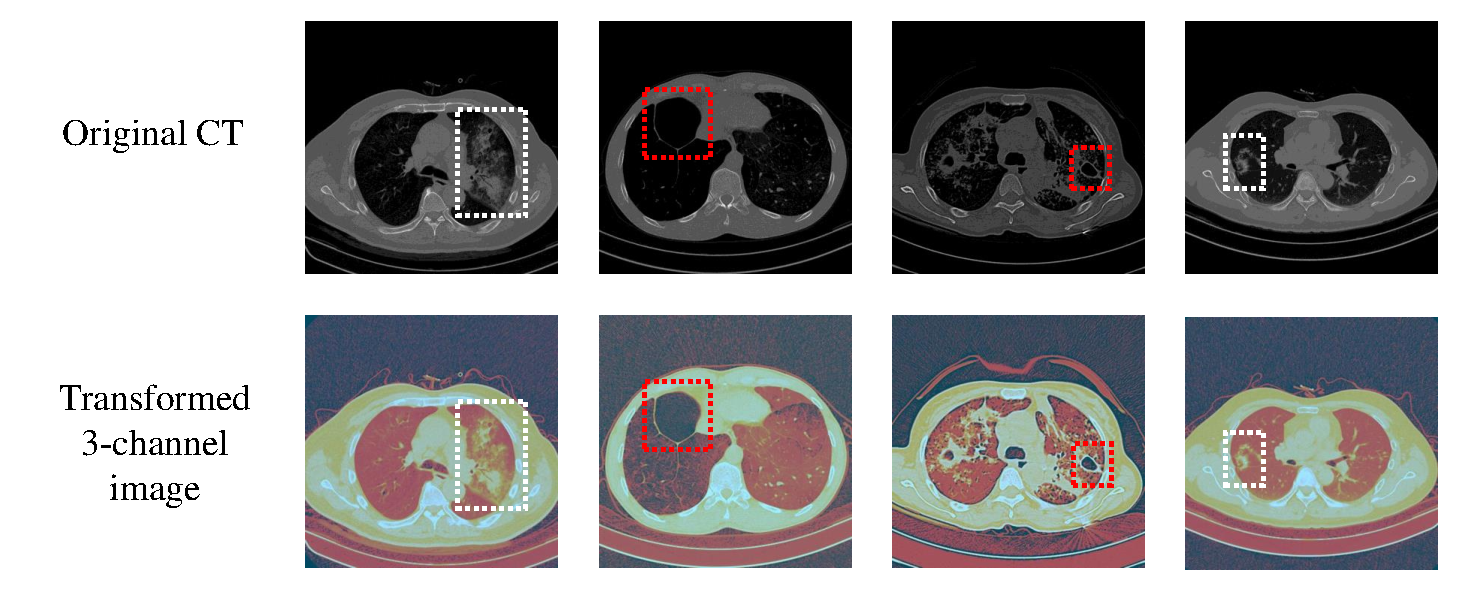
\includegraphics[width=5.5in]{3channel2.pdf}
    %\caption{fig2}
    \end{minipage}%
    }%
    \centering
    \caption{(a) shows data pre-process for CT scans. `slice i' represents i-th scan in the CT sequence. Each scan will be transformed into three images with different windows. Then three images will be compressed into one three-channel false-color image.
    (b) exhibit examples of three-channel images. We can see that void space (in red rectangle) in original CT images is not very obvious since other normal tissues are in black too. But in the three-channel images, we notice the difference between normal tissues and low dense tissues. Moreover, the details of high dense tissues (in the white rectangle) are still kept.
    }
    \label{3channel}
    \end{figure*}

As a result, 552 pneumonic cases and 450 cases of healthy people (1002 cases total) are left.
The dataset is divided into training / validation / testing as 60\% / 20\% / 20\% and make them identically distributed in three parts of datasets, so we have 602 cases in the training set, 200 cases in the validation set, 200 cases in the test set.
Each CT scan has a case file. In case files, we can get patient basic information: patient ID, gender, age, and chief complaint. 

\subsubsection{Pre-processing of CT Image Data}
\label{ctimagedata}
There are different kinds of image windows for CT reader, such as windows for bone, brain, chest, or lung. Images under different image windows will highlight different tissues of bodies.
As mentioned in section\ref{ctimagedata}, we can see that each series of CT has one specific `Convolution Kernel'. But it may make data inconsistent between different cases. So we transform raw data into HU(Hounsfield Unit) values. The Hounsfield Unit is a quantitative scale for describing radio-density. After transformed into HU value matrices, all slices form CT scans will have the same unit of measure.

Following the study in \cite{Shin2017Three, gao2018holistic}, HU value matrices will be transformed into images using three HU windows: Lung Window (LW) [-1000, 400HU], High Attenuation (HA) [-160, 240HU], Low Attenuation (LA) [-1400, -950HU]. 
For each slice, it will generate three one-channel grey level images. Then we compress three one-channel grey level images into one three-channel false-color RGB image. The `Slice Thickness' between each slice is adjusted into 10mm, and each case will keep 32 slices.

As shown in Fig~\ref{3channel}, we can see that three-channel images can show more density information about lung tissues. Original CT images are grey level images; high dense tissues are white; normal lung tissues and low dense tissues tend to be black. 
Relatively, three-channel false-color images have a larger scale of colors. First of all, high dense tissues will still tend to be white, like bones, high dense tissues in the lungs. Second, normal lung tissues will tend to be red, and low dense tissues tend to be black, which is very useful when patients have severe lung diseases.
The influence of different HU value ranges will be discussed in section~\ref{effectiveness}.
    
\subsubsection{Pre-processing of Patient Age, Gender and Chief Complaints}
\label{textdata}
Information about age and gender will be transformed into a two-dimensional array. For example, an adult male who was born in 1999-10-29 will have $[1, 20]$ to represent his information. A female patient born in 1993 will have $[0, 26]$ to indicate her information. The first dimension indicates gender, $1$ represents the male patient, $0$ represents the female patient. The second dimension represents the age of patient.

For patients' chief complaints, since all chief complaints are written in Chinese, we have to do Chinese word segmentation. Chinese word segmentation is a challenging problem, so we will take a short cut and use a mature tool: Jieba text segmentation $\footnote[1]{https://github.com/fxsjy/jieba}$ to segment Chinese sentences into Chinese word sequences.
After word-segmentation, we use word2vec \cite{mikolov2013efficient, mikolov2013distributed} to embed word sequences into vectors and use CBOW(Continuous Bag-of-Words) to capture relationship between words. Since our corpus is very small, the embedding size is set to 50, and the window size for CBOW is set to 3. We set length of Chinese word sequence to 16 since 16 is the maximum length among all chief complaint sequences. For those sequences whose length is less than 16, we add `None' to fill up the voids and increase the length to 16. The details of word2vec will not be discussed here. After embedding, each word will be embedded into a vector of 50 dimensions.


\section{Multimodal Pneumonia Detection Network }
\label{MPDNetwork}
\subsection{Construction of RCNN}
\label{RCNN}
RCNN (Recurrent Convolutional Neural Network) has been proved to be very effective in video caption, description, and classification \cite{Donahue2015Long, Aafaq2019Spatio}, some studies have applied RCNN to medical image analysis. Zreik, Majd et al. \cite{Zreik2018A} recently used RCNN for automatic detection and classification of coronary artery plaque, they used CNN extracts features out of $ 25\times25\times25$ voxels cubes and used an RNN to process the entire sequence using gated recurrent units (GRUs)\cite{chung2014empirical}. KL Tseng et al. \cite{tseng2017joint} exploited convolutional LSTM to model a sequence of 2D slices, and jointly learn the multi-modalities and convolutional LSTM in an end-to-end manner to segment 3D biomedical images.

As mentioned in section~\ref{intro}, CT allows visualization of lung structures, which brings a large amount of redundant information, like muscle, vessels, and bones. It will cost lots of calculation resource if we use 3D CNN directly. However, if we treat CT slices as short video frames, we can analyze them using RCNN. In RCNN, each slice will be fed into CNN in sequence and get a sequence of visual features. Then this sequence of features will be fed into RNN, so that we can reduce the need for calculation resource and keep 3D spatial information at the same time. 
Follow the study \cite{Donahue2015Long}, we use LSTM with $256$ units as our RNN cells cause LSTM has been demonstrated to be capable of large-scale learning of sequence data. 

We use CNN without fully-connected layers as a feature extractor. The input size of CNN is $512 \times 512$, so the outputs of CNN will be extensive. We use the global average pooling \cite{lin2014network} to reduce the number of neurons significantly. It is a replacement of fully-connected layers to enable the summing of spatial information of feature maps. After global average pooling, we insert a fully-connected layer to reduce dimensions to $256$ to fit the number of LSTM units.
To get the best RCNN for CT scans, after LSTM layer, we insert two additional fully-connected layers to give out classification results of RCNN, so that we can observe performances of different RCNNs and choose appropriate architecture. Experiments will be discussed later in section~\ref{experiments}.

After building RCNN, we will keep architecture above LSTM (including LSTM) and insert into our MPDNet as encoder of visual features. It encodes image feature sequences and gives out the last output of LSTM as middle state $hv_t$:
\begin{equation}
hv_t = LSTM(Fx_t, hv_{t-1}, z_{t-1})
\label{hvt}
\end{equation}
$Fx_t$ is the $t$-th visual features in CT slices, $hv_{t-1}$ is LSTM hidden state of $t-1$ step, $z_{t-1}$ is LSTM output of $t-1$ step. $t$ is the length of slices, in this study, we set $t$ as 32.

\subsection{Multimodal Data Fusion}
\label{MMDDtxt}

The whole RCNN, as mentioned in section~\ref{RCNN}, can be seen as an encoder of CT images.
Besides CT image information, we also have clinical information about patients gender, age, and chief complaints. 

Details of processing steps have been discussed in section~\ref{datasetprocessing}. The second LSTM is used to encode chief complaints. It is calculated in the same way as Eq.~\ref{hvt}:
\begin{equation}
    hc_{ct} = LSTM(Cx_{ct}, hc_{ct-1}, z_{ct-1})
    \label{hct}
\end{equation}
$Cx_{ct}$ is word embedding matrix of the $ct$-th word in chief complaint, $hc_{ct-1}$ is LSTM hidden state of $ct-1$ step. $ct$ is the length of chief complaint, which is 16. 

After getting $hv_t$, $hc_{ct}$, we can calculate the prediction and loss $\Phi_1$ as follows:
\begin{align*}\label{classifyandloss1}
    \Phi_1 &= \sum_i{y_i log(\Delta_i)}, \\
    \Delta &= Softmax(F(hv_t \bigotimes hc_{ct} \bigotimes A \bigotimes G))
\end{align*}
where $y_i$ are vectors for labels, $\Delta$ is prediction after Softmax layer, $\bigotimes$ is the concatenation operation, $A$ is patient age, $G$ is patient gender. $F$ is a function to calculate joint distributions of $hv_t$, $hc_{ct}$, $A$ and $G$. In this study, we use two fully-connected layers to fit the function. $\Phi_1$ is cross-entropy, which is commonly used as classification loss in many studies like \cite{Zreik2018A}.
\begin{table*}[htb]
    \caption{Comparison of All Kinds of RCNN and MPDNet}
    \begin{center}
    \begin{tabular}{|c|c|c|c|c|c|}

    \hline
    \textbf{\textit{Structure}} & \textbf{\textit{Data}}& \textbf{\textit{Accuracy}}  & \textbf{\textit{Sensitivity}} & \textbf{\textit{Specificity}} & \textbf{\textit{AUROC}}\\
    \hline
    RCNN(VGG) & Lung Window Image & 0.805 & {\bfseries 0.954} &0.626 &0.790 \\
    RCNN(GoogLeNet) & Lung Window Image& 0.865 & 0.826 & 0.912 & 0.869 \\
    RCNN(ResNet) & Lung Window Image & 0.925 & {\bfseries 0.954} & 0.890 & 0.922 \\
    RCNN(GoogLeNet) & High Attenuation Image& 0.880 & 0.853 & 0.912 & 0.883 \\
    RCNN(ResNet)& High Attenuation Image& 0.875 & 0.908 & 0.835 & 0.872 \\
    RCNN(GoogLeNet) & Low Attenuation Image& 0.860 & 0.890 & 0.824 & 0.857 \\
    RCNN(ResNet) & Low Attenuation Image& 0.865 & 0.900 & 0.824 & 0.861 \\
    RCNN(VGG) & Three Channel Image& 0.890 & 0.927 &0.846 &0.886 \\
    RCNN(GoogLeNet)& Three Channel Image & 0.905 & 0.900 & 0.912 & 0.906 \\
    RCNN(ResNet) & Three Channel Image& {\bfseries 0.930} & 0.927 &  {\bfseries 0.934} &  {\bfseries 0.930} \\
    RCNN(ResNet), One Loss & Three Channel Image& 0.920 & 0.917 & 0.923 & 0.920 \\
    \hline

    \end{tabular}
    \vspace{-0cm}
    \label{rcnncompare}
    \end{center}
    \vspace{-0cm}
    \end{table*}
Since each case has 32 slices but the loss is calculated for only one time in each case, we assume that the gradients propagate to CNN will be very weak, so that CNN will not be appropriately trained. Invoked by the study in \cite{szegedy2016rethinking}, we use an auxiliary loss to enhance the signal of the gradient for CNN.
The auxiliary loss $\Phi_2$ and loss of whole model $Loss$ are defined as follow: 
\begin{align*}
Loss &=  (1 - \omega) \times \Phi_1 +  \omega \times \Phi_2 \\
\Phi_2 &= \sum_i{y_i log(\Delta^c_i)}
\end{align*}
where $\omega$ is a parameter within the interval (0, 1). $\Phi_2$ is classification cross-entropy loss from CNN, $\Delta^c_i$ is Softmax prediction of CNN. $\omega$ can adjust the weight of two losses at different training phases.
We expect that at the beginning of training, CNN gets stronger gradient and learn to capture features from CT images more quickly. After parameters of CNN get stable, $\Phi_1$ tends to get small and keep updating parameters of LSTM. Experiments also show that RCNN with auxiliary loss can have a better performance, which will be discussed later in section~\ref{experiments}. The parameters in MPDNet are optimized by minimizing the $Loss$.


Finally, MPDNet, which simulates clinical pneumonia detecting process, is built. RCNN for image data and LSTM for clinical information will be trained jointly.


\section{Experiments}
\label{experiments}
\begin{figure*}[t]
    \centerline{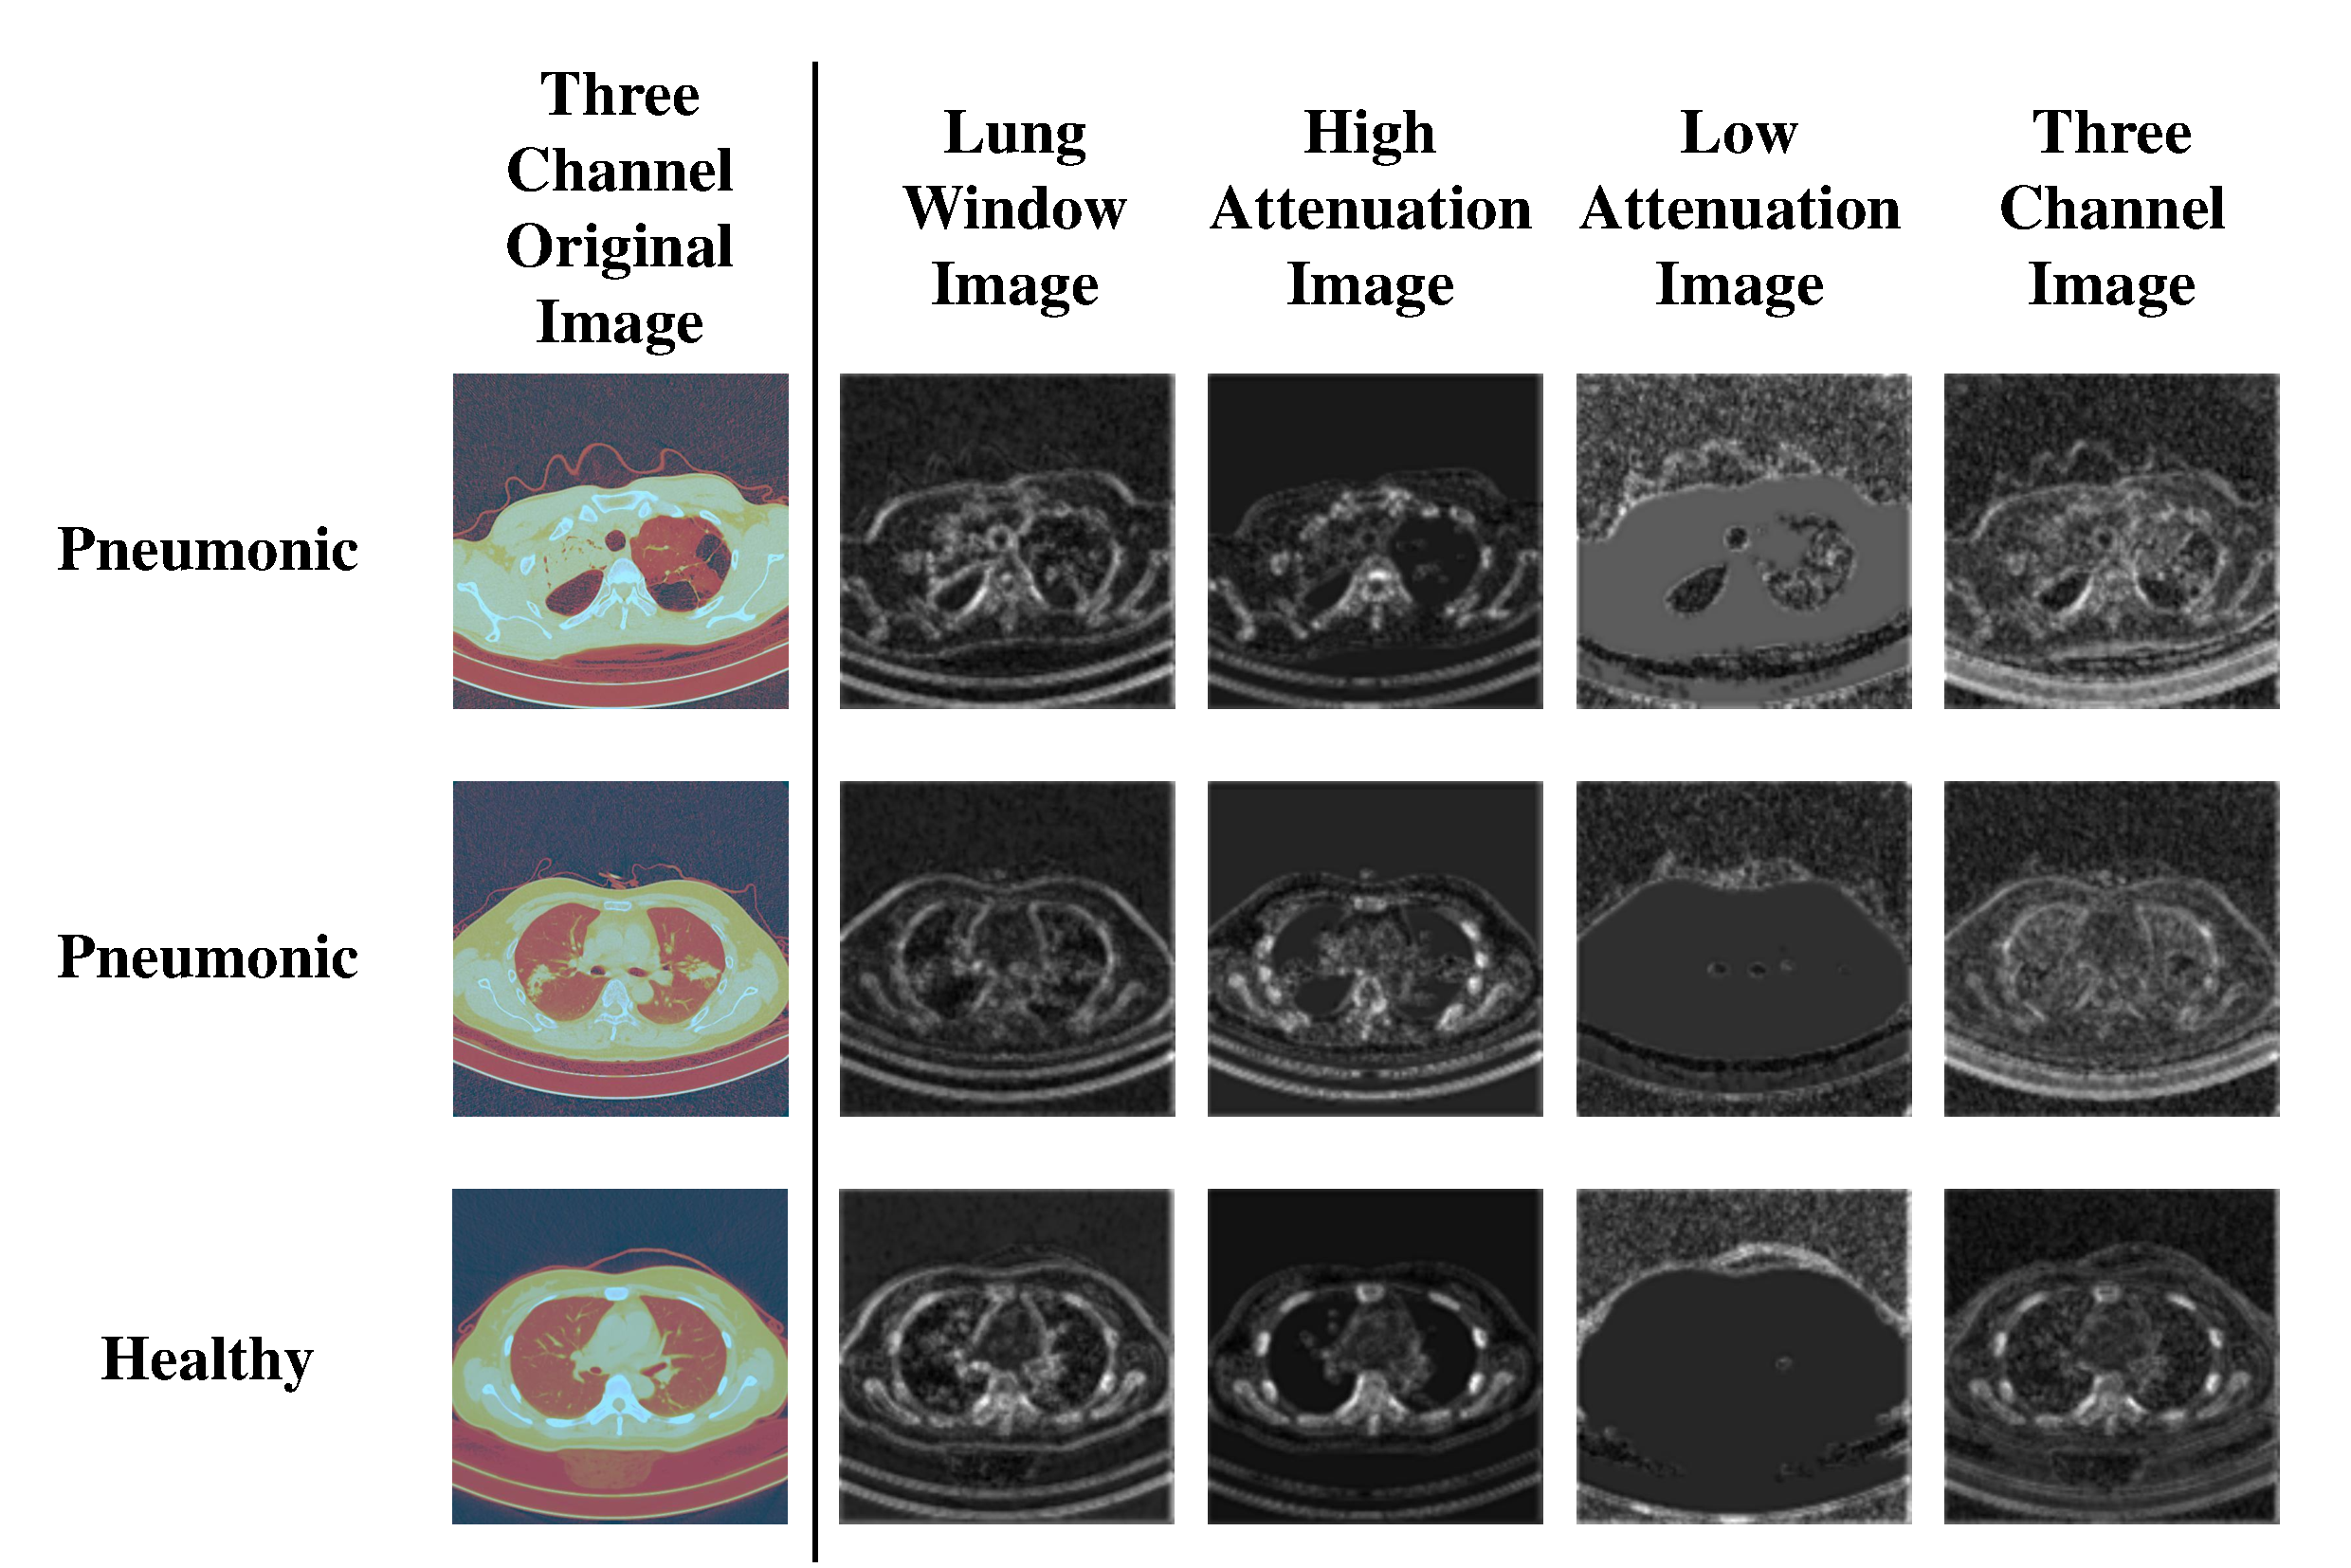
\includegraphics[width=150mm]{show.pdf}}
    \vspace{-0cm}
    \caption{Convolutional Feature Maps from CNN Models Trained by Different Images. In the first row, three-channel CNN can capture the low dense tissues of lungs, which are not very clear in LW (Lung Window) CNN and HA (High Attenuation) CNN. LA (Low Attenuation) CNN can notice the low dense tissues, but the details of heart and vessels are ignored in the low attenuation CNN. 
    In the second row, three-channel CNN still can capture high dense tissues, which is the same as LW CNN and HA CNN, but LA CNN has difficulty in doing so. The last row shows a healthy case. The healthy case has a clear view in LW CNN, HA CNN, and three-channel CNN, but shows nothing in LA CNN.}
    \vspace{-0cm}
    \label{show}
    \end{figure*}

\subsection{Experimental Setup}
\label{experimentalsetup}
There are two steps in the training process.
The first step is to train different kinds of RCNN networks to get the best combination between CNN and LSTM, the outputs from RCNN ($1 \times 256$) will be feed into two fully connected layers to get classification results. 
We test performances of different LSTM units numbers ($64$, $128$, $256$, $512$). Experiments show that $64$, $128$ and $256$ LSTM units have almost the same performances, they all get around 0.93 in accuracy, $512$ LSTM units only get 0.915 in accuracy. As a result, we follow the study \cite{Donahue2015Long} and set the number of LSTM units $256$.
Moreover, we use CNN models pre-trained on ImageNet \cite{ILSVRC15}. Experiments demonstrate that using pre-trained models can significantly improve the converging speed. 

The second step is to train the MPDNet model. We use RCNN as an encoder for CT scan visual features, use LSTM as an encoder for chief complaint features, and combine them with information of age and gender. All these features will be fed into two fully-connected layers and one Softmax layer to get final classification results. The initial learning rate is set to 0.0005 and drops 50\% every 3000 training steps. The dropout rate in fully-connected layers is set to 0.5. MPDNet will be trained for four epoch, and each epoch contains 15 iterations for all training data. In this work, all the experiments are run on the NVIDIA DGX Station with a GPU of NVIDIA Tesla V100. 

Source code for data pre-processing and MPDNet will be released very soon. We will also release the model with trained parameters and some sample cases for demo. But we cannot release dataset because of the privacy of patients. 

    
\subsection{Effect of Three-Channel Image and Auxiliary Loss}
\label{effectiveness}

In this section, we have conducted several experiments to
analyze the effect of the three-channel image and auxiliary loss. 
We test three kinds of classic CNN models: VGG16 \cite{simonyan2015very}, ResNet \cite{he2016deep} and GoogLeNet with Inception-V3 \cite{szegedy2016rethinking} with three-channel images, LW (Lung Window) images, HA (High Attenuation) images, and LA (Low Attenuation) images. Experiment results are shown in Table~\ref{rcnncompare}. 

We can see that RCNN(VGG) and RCNN(ResNet) trained by LW images perform better in sensitivity, but their specificity is lower than 0.9. ResNet50 trained by three-channel images performs the best in accuracy, specificity, AUROC.
These results demonstrate two phenomenons: (1) ResNet50 has a better performance on visual features learning than VGG16 and GoogLeNet with Inception-V3. This conclusion is similar to the conclusion drawn in \cite{Wang2017ChestX}, and their experiments showed that ResNet50 outperformed GoogLeNet and VGG16. (2) Three-channel images can provide more complete visual information of lungs. RCNN(ResNet), RCNN(VGG), and RCNN(GoogLeNet) trained with three-channel images have the best performances compared to these trained with LW, HA, and LA images. 
As a result, our RCNN use ResNet50 as its CNN part, and use one layer of LSTM cells as its RNN part. 

To experimentally analyse the effect of three-channel images, we output the feature maps of the convolutional layer, which are displayed in Fig~\ref{show}. More specificity, we output the feature maps after one convolutional layer, one max-pooling layer, and three ResNet blocks, the size of feature maps are $128 \times 128$. To keep experiments environment consistent, all experiments carried on in this part are based on RCNN with ResNet50. We can see that CNN trained by three-channel images has advantages over CNNs trained by other kinds of images. 
In Fig~\ref{show}, images in the first column are original false-color CT images, which are direct outputs from CT slices. The second, the third and the fourth columns are feature maps from LW CNN, HA CNN, and LA CNN. Images in the last column are feature maps from three-channel CNN. 
According to Fig~\ref{show}, HA window can keep high dense information, but HA has difficulty in capturing the difference between low dense tissues and normal tissues. Contrarily, LA can keep low dense information will, but high dense information tends to be blank in LA. LW window is close to the three-channel window. However, the three-channel window has better discrimination for normal tissues and low dense tissues.

Moreover, we run an experiment to prove the effect of auxiliary loss. We train RCNN(ResNet) with three-channel images, but we set $\omega$ to $1$, which means we remove the gradient propagates directly to CNN, this model has only one loss. We can see that the performance of RCNN with single loss drops around 1\% in all four indications. We also output weights of two losses during training and observe that weight for LSTM loss ($1 - \omega$) is 0.6238 at the beginning of training (602 steps), however, ($1 - \omega$) will increase to 0.7234 when training process comes to 36120 steps, it means weight for CNN is 0.3762 at 602 steps, and it will drop to 0.2766 at the end. These two phenomenons prove that, by using auxiliary loss, CNN will be trained in a better way. 

\subsection{Effect of Chief Complaints, Age and Gender}
\label{complaintsagegender}
In this section, we demonstrate the effect of clinical information.
As mentioned in section~\ref{intro}, information about age, gender, and chief complaints can enhance the features extracted from the CT image or become a supplement. Chief complaints can provide information like symptoms, location.
To verify that cheif complaints can provide symptoms which are related to pneumonia, we count word frequency about symptoms. The frequency is shown in Table~\ref{frequency1}. We can see that the top 10 keywords in HC (healthy cases) and PC (pneumonic cases) have certain regularity. `Cough' is the most frequent keyword in both HC and PC. It appears 256 times (46.4\%) in PC, 183 times (40.7\%) in HC. However, symptoms like `Expectoration', `Fever', `Coughing blood' appear more frequently in PC. For example, `Coughing blood' appears 47 times in PC, but only appears one time in HC. According to this table, patient who have symptoms like expectoration, repeat condition, shortness of breath have larger chance of having pneumonia. Patients who have chest pain, or feel unconfortable have less chance of having pneumonia. Having cough, on the other hand, is a symptom with minimal discrimination.

\begin{figure}[t]
    \centerline{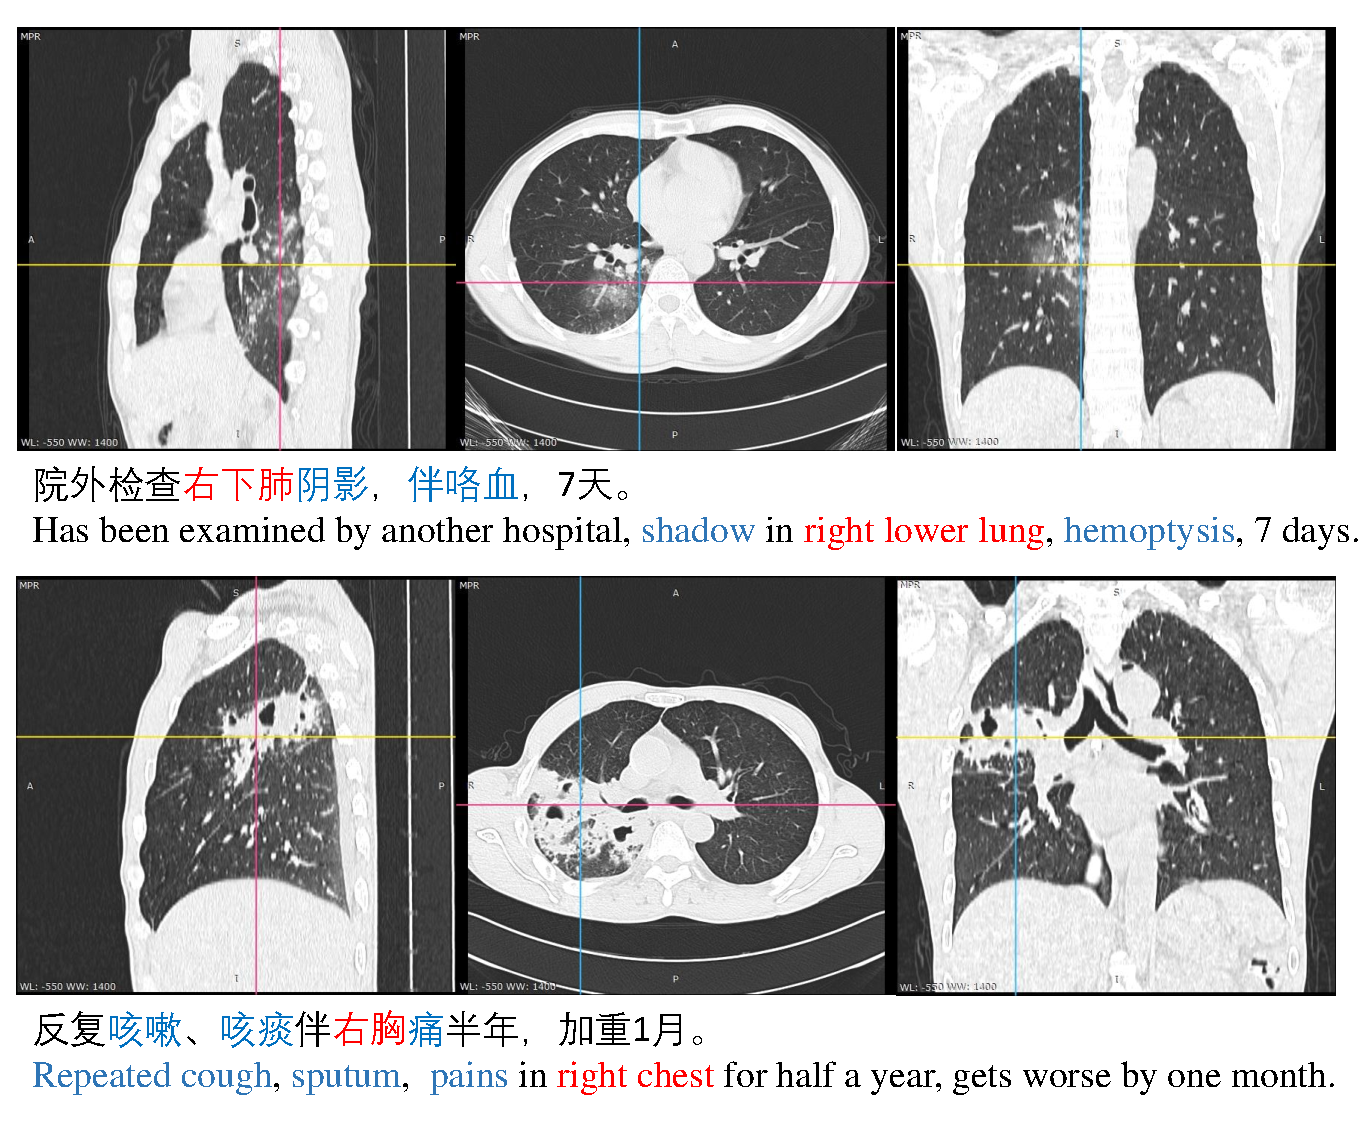
\includegraphics[width=90mm]{txtpic.pdf}}
    \vspace{-0cm}
    \caption{Chief complaints can provide information related to CT images. In this figure, we show two pneumonic cases, and each case has chief complaints provided by patients. Words marked red give the location, and words marked blue provide symptoms. English chief complaints are translated from Chinese above. We can see that location and symptoms information provided by chief complaints are related to abnormal tissues in CT images.}
    \vspace{-0cm}
    \label{txtpic}
    \end{figure}

\begin{table*}[htb]
    \vspace{-0cm}
\caption{}
\vspace{-0cm}
\begin{center}
\begin{tabular}{c|c|c|c|c}
\multicolumn{5}{c}{\textbf{Top 10 Frequent Key Words in Pneumonic Cases}} \\
\hline
    \textbf{\textit{Key Words}} & \textbf{\textit{Frequency in PC}} & \textbf{\textit{Percentage}}& \textbf{\textit{Frequency in HC}}& \textbf{\textit{Percentage}} \\
\hline
\begin{CJK}{UTF8}{gbsn}\textbf{咳嗽}\end{CJK}, \textbf{Cough} & 256 & 0.464 & 183 & 0.407\\
\begin{CJK}{UTF8}{gbsn}\textbf{咳痰}\end{CJK}, \textbf{Expectoration} & 103 & 0.187 & 42 & 0.093\\
\begin{CJK}{UTF8}{gbsn}\textbf{反复}\end{CJK}, \textbf{Repeat Condition} & 65 & 0.118 & 48 & 0.107\\
\begin{CJK}{UTF8}{gbsn}\textbf{气促}\end{CJK}, \textbf{Shortness of Breath} & 60 & 0.109 & 17 & 0.038\\
\begin{CJK}{UTF8}{gbsn}发热\end{CJK}, Fever & 51 & 0.092 & 14 & 0.031\\
\begin{CJK}{UTF8}{gbsn}咯血\end{CJK}, Coughing Blood & 47 & 0.085 & 1 & 0.002\\
\begin{CJK}{UTF8}{gbsn}加重\end{CJK}, Aggravation & 46 & 0.081 & 13 & 0.029\\
\begin{CJK}{UTF8}{gbsn}\textbf{痰}\end{CJK}, \textbf{Sputum} & 32 & 0.058 & 19 & 0.042\\
\begin{CJK}{UTF8}{gbsn}乏力\end{CJK}, Weak& 29 & 0.053 & 7 & 0.016\\
\begin{CJK}{UTF8}{gbsn}感染\end{CJK}, Infection& 28 & 0.051 & 1 & 0.002\\


\hline
\multicolumn{5}{c}{}\\
\multicolumn{5}{c}{\textbf{Top 10 Frequent Key Words in Healthy Cases}} \\
        \hline
        \textbf{\textit{Key Words}} & \textbf{\textit{Frequency in HC}} & \textbf{\textit{Percentage}}& \textbf{\textit{Frequency in PC}}& \textbf{\textit{Percentage}} \\
    \hline
    \begin{CJK}{UTF8}{gbsn}\textbf{咳嗽}\end{CJK}, \textbf{Cough},  & 183 & 0.407 & 256 & 0.464\\
    \begin{CJK}{UTF8}{gbsn}胸痛\end{CJK}, Chest Pain & 67 & 0.149 & 17 & 0.031\\
    \begin{CJK}{UTF8}{gbsn}不适\end{CJK}, Unconfortable & 54 & 0.120 & 25 & 0.045\\
    \begin{CJK}{UTF8}{gbsn}疼痛\end{CJK}, Pain & 53 & 0.118 & 25 & 0.045\\
    \begin{CJK}{UTF8}{gbsn}\textbf{反复}\end{CJK}, \textbf{Repeat Condition} & 48 & 0.107 & 65 & 0.118\\
    \begin{CJK}{UTF8}{gbsn}\textbf{咳痰}\end{CJK}, \textbf{Expectoration} & 42 & 0.093 & 103 & 0.187\\
    \begin{CJK}{UTF8}{gbsn}背痛\end{CJK}, Backache & 28 & 0.062 & 8 & 0.014\\
    \begin{CJK}{UTF8}{gbsn}\textbf{痰}\end{CJK}, \textbf{Sputum}& 19 & 0.042 & 32 & 0.058\\
    \begin{CJK}{UTF8}{gbsn}胸闷\end{CJK}, Chest Tightness & 19 & 0.042 & 16 & 0.029\\
    \begin{CJK}{UTF8}{gbsn}\textbf{气促}\end{CJK}, \textbf{Shortness of Breath}& 17 & 0.038 & 60 & 0.109\\
    
    \hline

\end{tabular}
\vspace{0.1cm}
\label{frequency1}\\
\footnotesize{Percentage is frequency divided by number of cases. PC is Pneumonic Cases. HC is Healthy Cases}

\end{center}
\vspace{-0cm}
\end{table*}
    

To verify that chief complaints can provide the location of the infection, we extract chief complaints with their CT images. Fig~\ref{txtpic} shows two examples. According to the location and symptom information provided by chief complaints, we can accurately locate lesions in CT. 
In these two cases, words marked red is information related to location, words marked blue are related to symptoms. In the first case, its chief complaint locates the symptoms in the right lower lung, and then we find shadows in the accurate place. In the second case, it chief complaint says that this patient has pains in right chest, then we also find shadows in the right lung in CT images.
This phenomenon demonstrates that information from chief complaints is related to CT images, and can assist deep learning model.

\subsection{Multimodal Pneumonia Detection Network}
\label{results}
In this section, the comprehensive evaluation of Multimodal Pneumonia Detection Network (MPDNet) is shown, results of experiments are shown in Table~\ref{mpdnetres}.
\begin{table*}[htb]
    \caption{Comparison of All Kinds of RCNN and MPDNet}
    \begin{center}
    \begin{tabular}{|c|c|c|c|c|c|}

    \hline
    \textbf{\textit{Structure}} & \textbf{\textit{Data}}& \textbf{\textit{Accuracy}}  & \textbf{\textit{Sensitivity}} & \textbf{\textit{Specificity}} & \textbf{\textit{AUROC}}\\
    \hline
    RCNN(ResNet) & Three Channel Image&  0.930 & 0.927 &  0.934 &  0.930 \\
    MPDNet & Three Channel Image \& Complaints & 0.925 & {\bfseries 0.945} & 0.901 & 0.923 \\
    MPDNet & Multimodal Data&  {\bfseries 0.945} & 0.936 & {\bfseries 0.956} & {\bfseries 0.945} \\
    \hline

    \end{tabular}
    \vspace{-0cm}
    \label{mpdnetres}
    \end{center}
    \vspace{-0cm}
    \end{table*}
As mentioned in section~\ref{MMDD}, the output of RCNN, features of chief complaints, gender, and age will be concatenated together and fused by two fully-connected layers. It is simple yet effective. We can see that MPDNet trained by multimodal data has the highest score in accuracy, specificity, and AUROC score. But it achieves 0.936 in sensitivity, 0.009 lower than the most top 0.945. It means MPDNet has the best performance of binary classification according to its AUROC score. 
Besides, we remove the information about age and gender and found that MPDNet without age and gender has a higher sensitivity and lower specificity than MPDNet with information about age and gender. 
    
If we treat RCNN(ResNet) trained with the three-channel image as our baseline, we can see that complaint information can increase sensitivity with 1.8\% to 94.5\%. It means chief complaints do have information which can help to detect pneumonia. Meanwhile, this information also decreases specificity to 90.1\%, which is not hard to understand cause patients sometimes cannot accurately describe his feelings or even exaggerate his condition. If we add information about age and gender, the sensitivity drops a little bit, but the specificity increases to 95.6\%, which means age and gender add information strongly connected to specificity.

The validation loss and accuracy during training is shown in Fig~\ref{loss}. We can see that MPDNet has the lowest loss and the highest accuracy during training.
According to Fig~\ref{loss}, we can see that information about age and gender can improve accuracy to 0.7 at the very beginning. It means some certain distribution must influence the dataset we are using. 
\begin{figure}[htbp]
    \centering
    \subfigure[Validation Loss During Training]{
    \begin{minipage}[t]{1\linewidth}
    \centering
    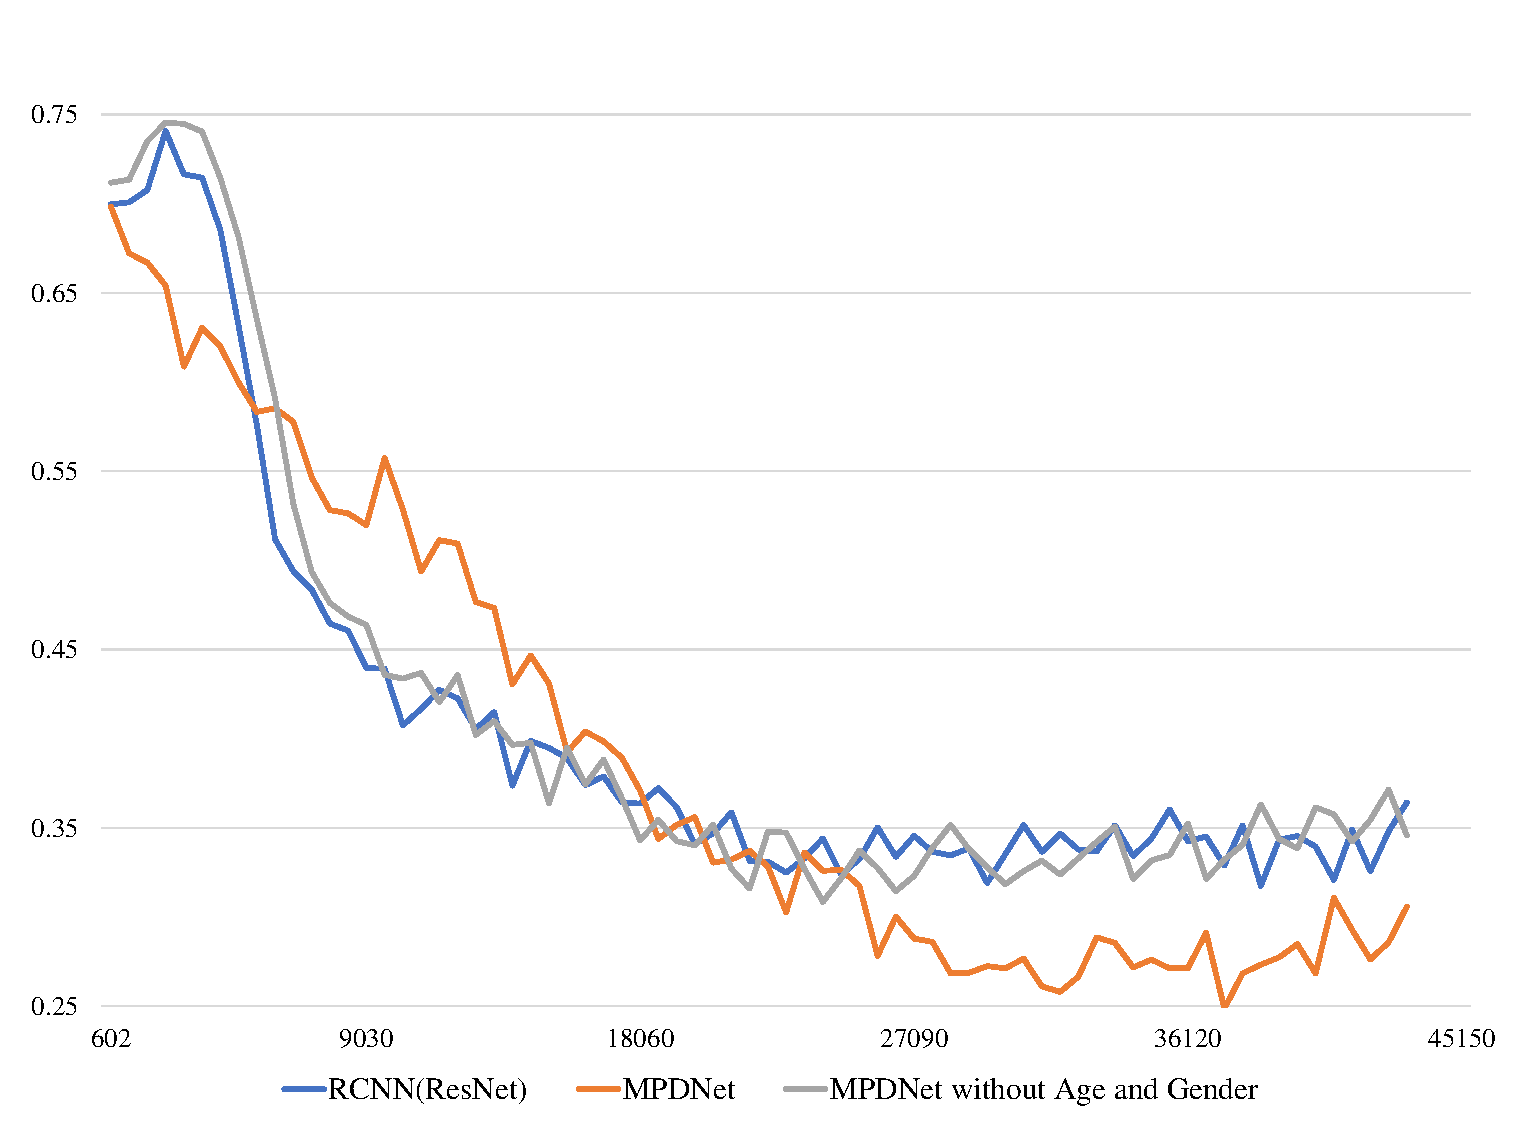
\includegraphics[width=3.5in]{trainloss.pdf}
    % \caption{Validation Loss During Training}
    \end{minipage}%
    }
    \subfigure[Validation Accuracy During Training]{
    \begin{minipage}[t]{1\linewidth}
    \centering
    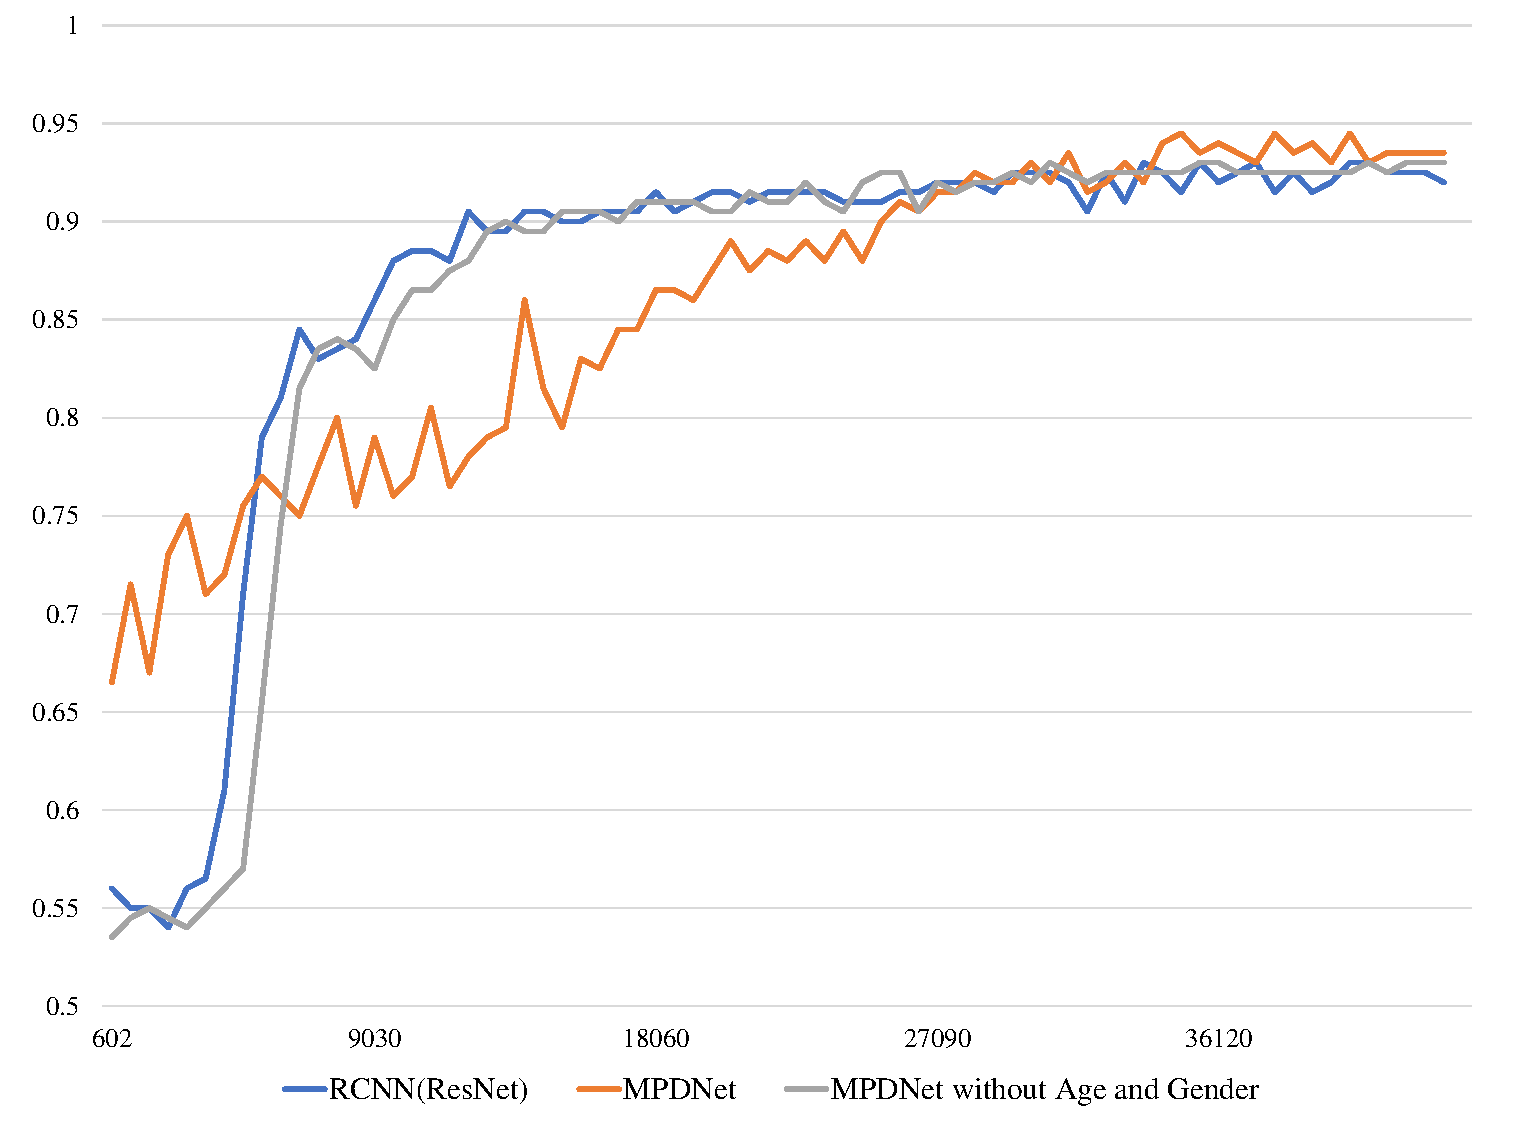
\includegraphics[width=3.5in]{trainacc.pdf}
    %\caption{fig2}
    \end{minipage}%
    }
    \centering
    \caption{(a) shows the validation loss during training; (b) shows the validation accuracy during training. We can see that MPDNet's performance outperforms others.
    }
    \label{loss}

    \end{figure}
So we count the number of male patients and female patients in healthy cases and pneumonic cases and the number of patients of different ages. 
In Table~\ref{malefemale}, (i) we can see that a male patient has a more significant chance of getting pneumonia. In 601 male cases, about 60\% of them are pneumonic; however, in 401 female cases, only 47.6\% are pneumonic. This phenomenon may be related to smoking since males in Chinese suffer a severe smoking problem; (2) The table shows that age is also associated with the chance of getting pneumonia. We can observe that people older than 40 have a much larger chance of getting pneumonia. There are about half of healthy cases between 40-50, but this indication drops so quickly that it goes down to 28.8\% between 50-60. These two tables explain why accuracy can achieve 0.7 at the very beginning of training and why information about age and gender can improve specificity to 95.6\%. These findings explain why priori information provided by gender and age can have such a remarkable effect on our network.

\begin{table}[htb]
    \vspace{-0cm}
    \caption{}
    \vspace{-0cm}
    \begin{center}
    \begin{tabular}{c|c|c|c|c}
    \multicolumn{5}{c}{\textbf{Number of Male and Female Patients in HC and PC}} \\
    \hline
    \textbf{\textit{}} & \textbf{\textit{Healthy}} & \textbf{\textit{Pneumonic}}& \textbf{\textit{Total}}& \textbf{\textit{Percentage*}} \\
    \hline
    Male & 240 & 361 & 601 & 60.1\%\\
    Female & 210 & 191 & 401 &47.6\% \\
    \hline
    \textbf{\textit{Total}} & 450 & 552 & 1002 & 55.1\% \\
    
    \hline
    \multicolumn{5}{c}{}\\
    \multicolumn{5}{c}{\textbf{Number of HC and PC in Different Ages}} \\

    \hline
    \textbf{\textit{}} & \textbf{\textit{Healthy}} & \textbf{\textit{Pneumonic}}& \textbf{\textit{Total}}& \textbf{\textit{Percentage*}} \\
    \hline
    0-10 & 6 & 1 & 7 & 14.3\%\\
    10-20 & 31 & 2 & 33 & 6.1\%\\
    20-30 & 122 & 30 & 152 & 19.7\%\\
    30-40 & 124 & 45 & 169 &26.6\%\\
    40-50 & 109 & 108 & 217 &49.8\%\\
    50-60 & 53 & 131 & 184 &71.2\%\\
    60-70 & 5 & 126 & 131 &96.2\%\\
    70-80 & 0 & 82 & 82 &100\%\\
    $>90$& 0 & 27 & 27 &100\%\\
    \hline 
    \textbf{\textit{Total}} & 450 & 552 & 1002 & 55.1\% \\

    \hline
    \end{tabular}
    \vspace{0.1cm}
    \label{malefemale} \\
    \footnotesize{Percentage* is Percentage of Pneumonia Patients}

    \end{center}

    \vspace{-0.0cm}
    \end{table}

\section{Discussion}
Even if MPDNet can detect pneumonia using multimodal data, there are still some shortcomings in our work.
Firstly, we analyze 1002 cases in this study. But 1002 cases are far small than `big data', so our model's performance is restricted by data distribution and quality. 
Secondly, we only consider chest CT scans, chief complaints, gender, and age. In clinical practice, besides the tests mentioned above, patients usually need to take blood pressure measurements, blood tests, heartbeat measurements, and other tests. These examinations can help doctors gain a more objective and comprehensive understanding of the patient condition so that doctors can make a more accurate diagnose.

However, it is very difficult to overcome these two shortcomings mentioned above since data collected from PACS are disorder. To construct a big scale medical dataset with consistent data is a very challenging task, cause raw data is affected by radiologists' habits, data acquisition equipment, and hospital work rules. 
Our future work will focus on finding a method which can perform accurate diagnose on disorder data and include multimodal information from more medical tests.

\section{Conclusion}
\label{conclude}
In this study, we propose a novel model MPDNet (Multimodal Pneumonia Detection Network), which combines CT visual features with patients' age, gender, and chief complaints to simulates clinical practice. 
MPDNet extracts visual features from three-channel images, semantic features from chief complaints, and fuses these features with priori information provided by age and gender.

We analyze 1002 cases (450 healthy cases and 552 pneumonic cases) from the Radiology Department of The First Affiliated Hospital of Army Medical University. Experiments demonstrate that MPDNet achieves promising performance.


% An example of a floating figure using the graphicx package.
% Note that \label must occur AFTER (or within) \caption.
% For figures, \caption should occur after the \includegraphics.
% Note that IEEEtran v1.7 and later has special internal code that
% is designed to preserve the operation of \label within \caption
% even when the captionsoff option is in effect. However, because
% of issues like this, it may be the safest practice to put all your
% \label just after \caption rather than within \caption{}.
%
% Reminder: the "draftcls" or "draftclsnofoot", not "draft", class
% option should be used if it is desired that the figures are to be
% displayed while in draft mode.
%
%\begin{figure}[!t]
%\centering
%\includegraphics[width=2.5in]{myfigure}
% where an .eps filename suffix will be assumed under latex, 
% and a .pdf suffix will be assumed for pdflatex; or what has been declared
% via \DeclareGraphicsExtensions.
%\caption{Simulation results for the network.}
%\label{fig_sim}
%\end{figure}

% Note that the IEEE typically puts floats only at the top, even when this
% results in a large percentage of a column being occupied by floats.


% An example of a double column floating figure using two subfigures.
% (The subfig.sty package must be loaded for this to work.)
% The subfigure \label commands are set within each subfloat command,
% and the \label for the overall figure must come after \caption.
% \hfil is used as a separator to get equal spacing.
% Watch out that the combined width of all the subfigures on a 
% line do not exceed the text width or a line break will occur.
%
%\begin{figure*}[!t]
%\centering
%\subfloat[Case I]{\includegraphics[width=2.5in]{box}%
%\label{fig_first_case}}
%\hfil
%\subfloat[Case II]{\includegraphics[width=2.5in]{box}%
%\label{fig_second_case}}
%\caption{Simulation results for the network.}
%\label{fig_sim}
%\end{figure*}
%
% Note that often IEEE papers with subfigures do not employ subfigure
% captions (using the optional argument to \subfloat[]), but instead will
% reference/describe all of them (a), (b), etc., within the main caption.
% Be aware that for subfig.sty to generate the (a), (b), etc., subfigure
% labels, the optional argument to \subfloat must be present. If a
% subcaption is not desired, just leave its contents blank,
% e.g., \subfloat[].


% An example of a floating table. Note that, for IEEE style tables, the
% \caption command should come BEFORE the table and, given that table
% captions serve much like titles, are usually capitalized except for words
% such as a, an, and, as, at, but, by, for, in, nor, of, on, or, the, to
% and up, which are usually not capitalized unless they are the first or
% last word of the caption. Table text will default to \footnotesize as
% the IEEE normally uses this smaller font for tables.
% The \label must come after \caption as always.
%
%\begin{table}[!t]
%% increase table row spacing, adjust to taste
%\renewcommand{\arraystretch}{1.3}
% if using array.sty, it might be a good idea to tweak the value of
% \extrarowheight as needed to properly center the text within the cells
%\caption{An Example of a Table}
%\label{table_example}
%\centering
%% Some packages, such as MDW tools, offer better commands for making tables
%% than the plain LaTeX2e tabular which is used here.
%\begin{tabular}{|c||c|}
%\hline
%One & Two\\
%\hline
%Three & Four\\
%\hline
%\end{tabular}
%\end{table}


% Note that the IEEE does not put floats in the very first column
% - or typically anywhere on the first page for that matter. Also,
% in-text middle ("here") positioning is typically not used, but it
% is allowed and encouraged for Computer Society conferences (but
% not Computer Society journals). Most IEEE journals/conferences use
% top floats exclusively. 
% Note that, LaTeX2e, unlike IEEE journals/conferences, places
% footnotes above bottom floats. This can be corrected via the
% \fnbelowfloat command of the stfloats package.






% if have a single appendix:
%\appendix[Proof of the Zonklar Equations]
% or
%\appendix  % for no appendix heading
% do not use \section anymore after \appendix, only \section*
% is possibly needed

% use appendices with more than one appendix
% then use \section to start each appendix
% you must declare a \section before using any
% \subsection or using \label (\appendices by itself
% starts a section numbered zero.)
%


% \appendices
% \section{Proof of the First Zonklar Equation}
% Appendix one text goes here.

% % you can choose not to have a title for an appendix
% % if you want by leaving the argument blank
% \section{}
% Appendix two text goes here.


% use section* for acknowledgment


% Can use something like this to put references on a page
% by themselves when using endfloat and the captionsoff option.
\ifCLASSOPTIONcaptionsoff
  \newpage
\fi



% trigger a \newpage just before the given reference
% number - used to balance the columns on the last page
% adjust value as needed - may need to be readjusted if
% the document is modified later
%\IEEEtriggeratref{8}
% The "triggered" command can be changed if desired:
%\IEEEtriggercmd{\enlargethispage{-5in}}

% references section

% can use a bibliography generated by BibTeX as a .bbl file
% BibTeX documentation can be easily obtained at:
% http://mirror.ctan.org/biblio/bibtex/contrib/doc/
% The IEEEtran BibTeX style support page is at:
% http://www.michaelshell.org/tex/thebibliography/bibtex/
\bibliographystyle{IEEEtran}
% argument is your BibTeX string definitions and bibliography database(s)
\bibliography{refs}
%
% <OR> manually copy in the resultant .bbl file
% set second argument of \begin to the number of references
% (used to reserve space for the reference number labels box)





% biography section
% 
% If you have an EPS/PDF photo (graphicx package needed) extra braces are
% needed around the contents of the optional argument to biography to prevent
% the LaTeX parser from getting confused when it sees the complicated
% \includegraphics command within an optional argument. (You could create
% your own custom macro containing the \includegraphics command to make things
% simpler here.)
%\begin{IEEEbiography}[{\includegraphics[width=1in,height=1.25in,clip,keepaspectratio]{mshell}}]{Michael Shell}
% or if you just want to reserve a space for a photo:

% \begin{IEEEbiography}{Michael Shell}
% Biography text here.
% \end{IEEEbiography}

% if you will not have a photo at all:
\newpage

\begin{IEEEbiography}[{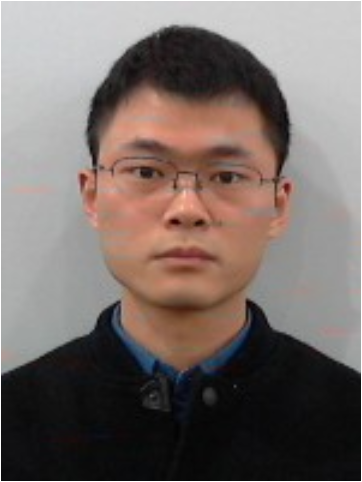
\includegraphics[width=1in,height=1.25in,clip,keepaspectratio]{qiuliwang.png}}]{Qiuli~Wang}
    received the B.E. degree in the School of Information Engineering, Yangzhou University in 2016. He is currently working toward the Ph.D. degree in the School of Big Data \& Software Engineering, Chongqing University. 
    
    His research interests include medical image computing, deep learning, so on.
\end{IEEEbiography}

\vspace{-0.5cm}

\begin{IEEEbiography}[{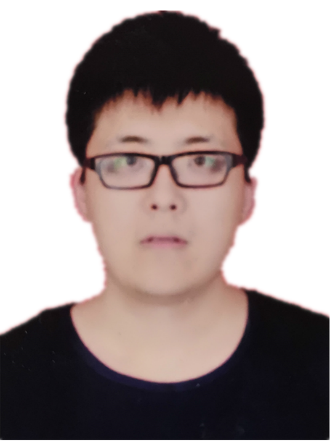
\includegraphics[width=1in,height=1.25in,clip,keepaspectratio]{zhihuanli.png}}]{Zhihuan~Li}
    received the B.E degree in Geological Engineering from China University of Mining and Technology, Xvzhou, China in 2016. He is currently working toward the M.S. degree in Software Engineering from the Department of Big Data \& Software Engineering, Chongqing University, Chongqing.
	His research interests include medical image analysis , segmentation and so on.
\end{IEEEbiography}

\vspace{-0.5cm}
\begin{IEEEbiography}[{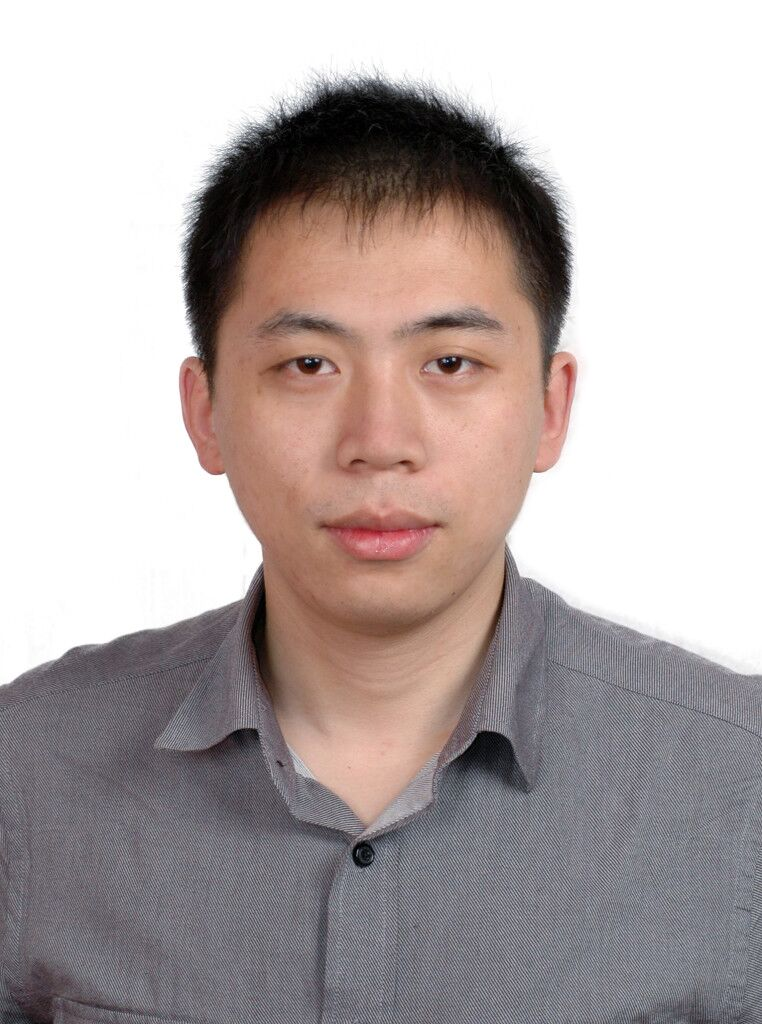
\includegraphics[width=1in,height=1.25in,clip,keepaspectratio]{chenliu.png}}]{Chen~Liu}
    received the M.D. degree in Medical Imaging from Army Medical University, China, in 2015. He is currently an attending physicians in the Radiology Department of Southwest Hospital which is the first affiliated hospital of Army Medical University. He has hosted more than 6 research including National Natural Science Foundation and got funded more than 1.6 million. He published 6 articles as first author. His current research interests include brain functional MRI, clinical data mining, medical imaging deep learning.
\end{IEEEbiography}




\vspace{-0.5cm}

\begin{IEEEbiography}[{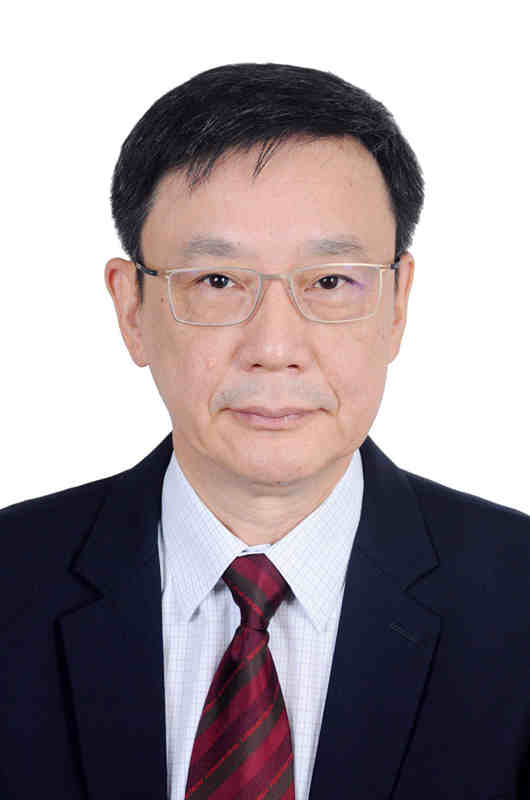
\includegraphics[width=1in,height=1.25in,clip,keepaspectratio]{danyang.png}}]{Dan~Yang}
    received the B.Eng. degree in automation, the M.S. degree in applied mathematics, and the Ph.D. degree in machinery manufacturing and automation from Chongqing University, Chongqing. From 1997 to 1999, he held a post-doctoral position with the University of Electro-Communications, Tokyo, Japan. He is currently the President of Southwest Jiaotong University. He is also a Professor with the School of Big Data \& Software Engineering, Chongqing University. He has authored over 100 scientific papers and some of them are published in some authoritative journals and conferences, such as the IEEE TRANSACTIONS ON PATTERN ANALYSIS AND MACHINE INTELLIGENCE, CVPR, and BMVC. His research interests include computer vision, image processing, pattern recognition, software engineering,
and scientific computing.
\end{IEEEbiography}
\vspace{-0.5cm}

\begin{IEEEbiography}[{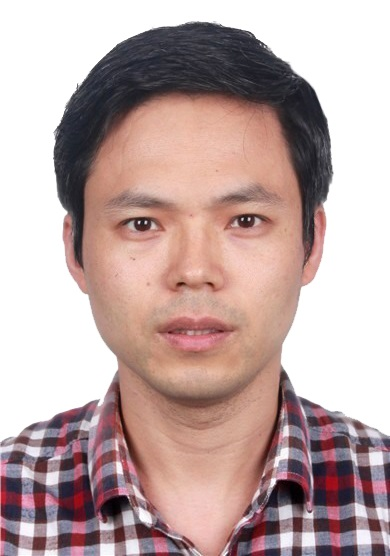
\includegraphics[width=1in,height=1.25in,clip,keepaspectratio]{xiaohongzhang.png}}]{Xiaohong~Zhang}
    received the M.S. degree in applied mathematics from Chongqing University, China, where he also received the Ph.D. degree in computer software and theory, in 2006. He is currently a Professor and the Vice Dean with the School of Big Data \& Software Engineering, Chongqing University. His current research interests include data mining of software engineering, topic modeling, image semantic analysis, and video analysis.
\end{IEEEbiography}
\vspace{-0.5cm}

% insert where needed to balance the two columns on the last page with
% biographies
%\newpage

% \begin{IEEEbiographynophoto}{XXX}
%     XXX
% \end{IEEEbiographynophoto}

% You can push biographies down or up by placing
% a \vfill before or after them. The appropriate
% use of \vfill depends on what kind of text is
% on the last page and whether or not the columns
% are being equalized.

%\vfill

% Can be used to pull up biographies so that the bottom of the last one
% is flush with the other column.
%\enlargethispage{-5in}



% that's all folks
\end{document}


